\documentclass{beamer}
\usepackage[utf8]{inputenc}
\usepackage{zxjatype}
\usepackage[ipa]{zxjafont}
\usetheme{metropolis}           % Use metropolis theme

\usepackage{ascmac}
\metroset{numbering=fraction}
\usepackage{my-default}

\title{MetropolisでDeepLearningいろいろ数式を書いてみる}
\author{竹川}

\usepackage{url}

%% おまじない
\newlength{\mytotalwidth}
\mytotalwidth=\dimexpr\linewidth-5mm
\newlength{\mycolumnwidth}
\mycolumnwidth=\dimexpr\mytotalwidth-5mm

%% ソースコードキャプション設定
\usepackage{minted}
\usemintedstyle{monokai}
\definecolor{LightGray}{gray}{0.9}


%% tikz設定
\usepackage{tikz}
\usetikzlibrary{arrows.meta}
\tikzset{%
  >={Latex[width=2mm,length=2mm]},
  % Specifications for style of nodes:
            base/.style = {rectangle, rounded corners, draw=black,
                           minimum width=4cm, minimum height=1cm,
                           text centered, font=\sffamily},
  activityStarts/.style = {base, fill=blue!30},
       startstop/.style = {base, fill=red!30},
    activityRuns/.style = {base, fill=green!30},
         process/.style = {base, minimum width=2.5cm, fill=orange!15,
                           font=\ttfamily},
}

\date{\today}
\begin{document}
\maketitle

あああ

\end{document}

%\part{ DeepLearning入門 No.1}


\section{Chapter 1 Intoroduction}
\begin{frame}{この章の目標}
講座全体のイントロと前提知識の確認
\begin{itemize}
    \item 機械学習とは?
    \item 数学
    \item  プログラミング
\end{itemize}
\end{frame}


\begin{frame}{この講座の目的}
理想は論文を読み、以下を理解する.
\begin{itemize}
    \item 提案手法特徴の理解
    \item 提案手法のアルゴリズム
    \item 提案手法の実装
\end{itemize}
つまり... \textbf{DeepLearning}になれる!!!!
\end{frame}


\begin{frame}{皆さんへのお願い}
皆さんの知識に合わせ、最適な授業にしたい
\begin{itemize}
    \item わからない点を質問してください \\
          一日最低3質問以上
   \item なるべくアウトプットを多くしていただく
\end{itemize}
\end{frame}



\begin{frame}{お願いその2}
現状は基本となる知識を教える想定なので,
仕事でDLしている方は予め教えて下さい...
もし多数であれば以下を解説する回があるかも
\begin{itemize}
    \item 理論系の論文
    \item NLP,画像処理,音声等の応用系の新しい論文
    \item 万能近似定理等の証明
\end{itemize}
\end{frame}

\begin{frame}{確認1 数学の知識}
多変数の合成関数の微分ができれば問題ありません. \\

\textbf{キーワード}
\begin{itemize}
  \item ベクトル
  \item 行列
  \item 合成関数の微分
  \item 多変数の微分
\end{itemize}
\end{frame}


\begin{frame}{確認2 Pythonの知識}
キーワード
\begin{itemize}
  \item if, for 等の最低限の文法
  \item 配列,dict
  \item numpyの知識
  \item Pytorchの手法
\end{itemize}
\end{frame}


\begin{frame}{確認3 Pythonの環境}
\begin{itemize}
    \item Kaggleのアカウント及びKernel \\
    Notebook等の共有はKaggle上で行いますので、まだ作れていない方は作って下さい.
    \item Google Colaboratory \\
    一部のGPUが必要なコードなどははここで確認してください.
    \item LocalのPython環境 \\
    あると便利ですが、必須ではありません.
\end{itemize}
\end{frame}


\begin{frame}{初学者向けのお願い}

私からのお願いです.
\begin{itemize}
\item 間違ってもいいので、トライしてください.
\item わからない原因を分析してください.
\item わからない箇所を検索してください.
\item 曖昧さを楽しみつつ、厳密さをこだわってください.
\end{itemize}
\end{frame}


Kaggleのアカウント作成タイム

https://www.kaggle.com/t/d646a2a5bb1c4ebda09639bffd4c252f

\section{人工知能と機械学習の歴史}

\begin{frame}{人工知能とは}
\begin{itemize}
\item 正確な統一された定義はない.
\item 直感的には"人の知能"を機械が学習するもの
\item 詳細は教科書を確認ください.
\end{itemize}
\end{frame}


\begin{frame}{かつては}
実行知能といえば\textbf{エキスパートシステム}のことだった.
エキスパートシステムの概要は
\begin{itemize}
  \item データから人間が特徴を見つけ出し
  \item その特徴を実装する
\end{itemize}
しかし,特徴を見つけ出すことに限界があった
\end{frame}


\begin{frame}{現在の人工知能}
人工知能の基本的方針
\begin{itemize}
\item データから学習するもの
\item 実質、機械学習
\end{itemize}
\end{frame}


\begin{frame}{機械学習}
\begin{itemize}
\item データから学習する能力を持つプログラム
\item かつては下火だった.
\item DLの大成功で台頭する.
\end{itemize}
\end{frame}


\begin{frame}{両者の違い}
\begin{itemize}
\item 人工知能 \\
      知能の代替が実現できれば方式は問わない
\item 機械学習
      \\ データを用いてパラメータをチューニングするアルゴリズム全般
\end{itemize}
\end{frame}


\section{機械学習とその分類}


\begin{frame}機械学習の登場人物
\begin{itemize}
\item データ: 機械学習の世界ではデータは数値です。
\item 仮説空間: データから予測する"関数"を仮説と言います。仮説空間は仮説 (関数) の集まりです。
\item 損失: 仮説の良し悪しを測るもの.
\end{itemize}
機械学習はデータを使い,指標が最小になるように,仮説空間を探索する.
\end{frame}


\begin{frame}{機械学習の種類}
\begin{itemize}
\item 教師あり学習: データが入力と出力の組
\item 教師なし学習: データが入力のみ
\end{itemize}
\end{frame}


\begin{frame}{教師あり学習の例}
メールをスパムが判定する問題
\begin{itemize}
\item 入力データ: メールに特定の文字があるか
\item 出力データ: スパムかどうか
\end{itemize}
\end{frame}


\begin{frame}{教師あり学習の例2}
建物の価格推定
\begin{itemize}
\item 入力データ: 広さ、地域、築
\item 出力データ: 建物の価格
\end{itemize}
\end{frame}


\begin{frame}{分類問題と回帰問題}
\begin{itemize}
\item 分類問題 (classification) : 離散変数の予測
\item 回帰問題 (regression) : 連続変数の予測
\item スパム判定は分類
\item 価格推定は回帰
\end{itemize}
\end{frame}


\begin{frame}{連続変数とは}
\begin{itemize}
\item 価格も整数なので離散なのでは?
\item 連続関数は関数に対して連続性を定義したものだったが?
\item 実際は値の大小に意味がある、かつ量がそれなり(問題依存)の時\textbf{連続}という.
\end{itemize}
\end{frame}


\begin{frame}{教師なし学習の例}
\begin{itemize}
\item 入力データ:顧客の商品購入履歴
\item 顧客の属性を5種類に分け分析する
\end{itemize}
\end{frame}


\begin{frame}{教師なし学習の特徴}
5種類の分割の解釈が機械任せ
\begin{itemize}
  \item 例えば、年齢ごとで5分割されるかもしれない
  \item 例えば、よく買うカテゴリーで分割されるかもしれない.
  \item たいていの場合、それらが曖昧で何を表すか読み解くのが困難
\end{itemize}
\end{frame}


\section{教師あり学習}


\begin{frame}{分類問題}
\begin{itemize}
\item 入力をいくつかに分割することに相当
\item その分割の境界を決定境界という.
\item 決定境界には線形と非線形がある.
\end{itemize}
\end{frame}


\begin{frame}{線形分類モデルの例}
\begin{itemize}
\item ソフトマックス回帰モデル
\item 線形サポートベクトル分類器
\end{itemize}
\end{frame}


\begin{frame}{非線形の例}
\begin{itemize}
\item k-近傍法
\item RBF カーネルによるサポートベクトル分類器
\item 3層以上のニューラルネットワーク
\item 決定木ベースの分類モデル
\item ガウス過程
\end{itemize}
\end{frame}


\begin{frame}{線形と非線形の違い}
\begin{itemize}
\item 線形の方が単純
  \begin{itemize}
  \item 最低限の精度が出やすい
  \item チューニングが簡単
  \end{itemize}
\item 非線形の方が複雑
  \begin{itemize}
  \item 計算に時間がかかる
  \item チューニングが難しい場合が多い.
  \end{itemize}
\end{itemize}
\end{frame}


\begin{frame}{ノーフリーランチ定理}
どんなタスクにも上手くいくような機械学習モデルというのは基本ない.
\end{frame}


\begin{frame}{演習}
\url{https://tutorials.chainer.org/ja/Exercise_Step_01.html}
\begin{itemize}
\item 2章
\item 4章
\end{itemize}
\end{frame}

\section{ノーフリーランチ定理の証明}
%\section{Chapter 4 DeepNeuralNetwork}


\begin{frame}[fragile]{ここで話すこと}
\begin{itemize}
\item  ニューラルネットワークのイメージ \\
\item ニューラルネットワークの定義 \\
\item ニューラルネットワークの表現能力 \\
\item ニューラルネットワークの学習 \\
\item DeepLearningのチューニング
\end{itemize}
\end{frame}

\section{AND/ORでみるニューラルネットワーク}

\begin{frame}{ニューラルネットワークの絵}
\begin{center}
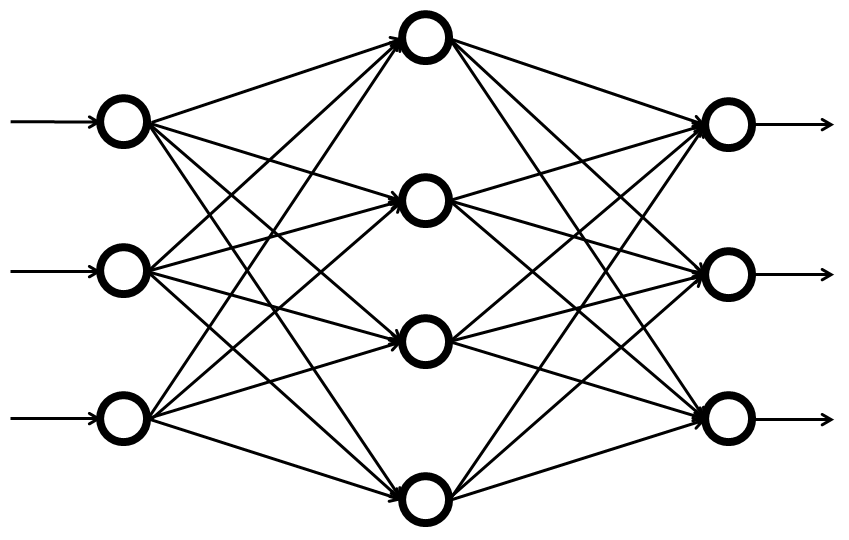
\includegraphics[width=8cm]{pic/dnn_sample.png}
\end{center}

\footnote{\url{http://nkdkccmbr.hateblo.jp/entry/2016/10/06/222245}より}
\end{frame}

\begin{frame}[fragile]{ニューラルネットワークの雰囲気}
  \begin{itemize}
    \item $\bullet$: ユニット
    \item $\bullet$の列: 層
    \item 層を重ねて予測をする.
  \end{itemize}
\end{frame}

\begin{frame}[fragile]{二層のパーセプトロンの定義}

\begin{screen}
\begin{dfn}
以下を満たすものを二層のパーセプトロンといいます.
\begin{itemize}
\item 入力: $x_1, x_2$
\item パラメータ: $w_1, w_2, \theta$
\item 出力:
\begin{equation*}
y = \left\{
\begin{array}{ll}
0 & w_1 x_1 + w_2 x_2 < \theta \\
1 & w_1 x_2 + w_2x_2 \ge \theta
\end{array}
\right.
\end{equation*}
\end{itemize}
\end{dfn}
\end{screen}
\end{frame}


\begin{frame}[fragile]{二層のパーセプトロンの性質}
\begin{itemize}
\item 実現できるもの
  \begin{itemize}
  \item AND
  \item OR
  \item NAND
  \end{itemize}
\item 実現できないもの
   XOR
\end{itemize}

\textbf{注意}: 入力は0,1のみを考える
\end{frame}

\begin{frame}[fragile]{AND}

実現例
\begin{itemize}
  \item $w_1 = w_2 = 0.5$
  \item $\theta = 0.7$
\end{itemize}

実際計算してみる
\begin{itemize}
\item $(x_1, x_2)$が(0,0),(1,0),(0,1)のときは高々0.5
\item (1,1)のときは1となります.
\item $\theta$の条件を考えると確かに`AND`.
\end{itemize}

\end{frame}

\begin{frame}[fragile]{OR}

実現例
\begin{itemize}
  \item $w_1 = w_2 = 0.5$
  \item $\theta = 0.3$
\end{itemize}
実際計算してみると

\begin{itemize}
\item $(x_1, x_2)$が(1,1),(1,0),(0,1)のときは少なくとも0.5
\item (0,0)のときは0となります.
\item $\theta$の条件を考えると確かに`OR`.
\end{itemize}
\end{frame}


\begin{frame}[fragile]{NAND}
NANDはANDを反転させたもの. \\
実現例
\begin{itemize}
  \item $w_1 = w_2 = -0.5$
  \item $\theta = - 0.7$
\end{itemize}
\end{frame}


\begin{frame}[fragile]{二層のパーセプトロンの気持ち}
\begin{itemize}
\item 二層のパーセプトロンは超平面で分離する = 線形モデル.
\item AND/NAND/OR等のモデルはかける
\item XORのような非線形なものはかけない
\end{itemize}
\end{frame}

\begin{frame}[fragile]{XOR}
XOR: $ \{0, 1\} \times  \{0, 1\} \to  \{0, 1\}$
\begin{itemize}
  \item $(0, 1), (1, 0)$の時1
  \item $(1, 1),(0, 0)$の時0
\end{itemize}

XOR二層のパーセプトロンでは表せない \\
もし表せたとすると,矛盾することを示します.
\end{frame}


\begin{frame}[fragile]{XORが表せない証明}
$(1, 0),(0, 1)$で$w_1x_1 + w_2x_2 \ge \theta$
\begin{itemize}
    \item $(1, 0)$の時$w_1 \ge \theta$
    \item $(0, 1)$の時$w_2 \ge \theta$
\end{itemize}
$(0, 0),(1, 1)$で$w_1x_1 + w_2x_2 < \theta$
\begin{itemize}
\item $(0, 0)$の時,$0 < \theta$
\item $(1, 1)$の時,$w_1 + w_2 < \theta$
\end{itemize}

この時、$w_1 \ge \theta$,$w_2 \ge \theta$より
\begin{itemize}
\item $w_1 + w_2 \ge 2\theta$となり,$0 < \theta$より
\item $w_1 + w_2 \ge 2 \theta  > \theta$となり
\end{itemize}
$(1,1)$の場合に条件と矛盾する.
\end{frame}


\begin{frame}[fragile]{三層での表現方法}
ただし、これを三層のパーセプトロンにすれば実現できます.

\begin{equation*}
\begin{array}{ll}
s_1 =  NAND(x_1, x_2) \\
s_2 =  OR(x_1, x_2) \\
XOR(x_1, x_2) = AND(s_1, s_2)
\end{array}
\end{equation*}
\end{frame}


\begin{frame}[fragile]{XORの結果の確認}
\begin{itemize}
\item (1,1)のとき
  \begin{itemize}
  \item $s_1 = NAND(1,1) = 0, s_2 = OR(1, 1) = 1$
  \item $AND(s_1, s_2) = AND(0, 1) = 0$
  \end{itemize}
\item (1,0)のとき
  \begin{itemize}
  \item $s_1 = NAND(1,0) = 1, s_2 = OR(1, 0) = 1$
  \item $AND(s_1, s_2) = AND(1, 1) = 1$
  \end{itemize}
\item (0,1)のとき
  \begin{itemize}
  \item $s_1 = NAND(0,1) = 1, s_2 = OR(0, 1) = 1$
  \item $AND(s_1, s_2) = AND(1, 1) = 1$
  \end{itemize}
\item (0,0)のとき
  \begin{itemize}
  \item $s_1 = NAND(0,0) = 1, s_2 = OR(0, 0) = 0$
  \item $AND(s_1, s_2) = AND(1, 0) = 0$
  \end{itemize}
\end{itemize}
\end{frame}


\begin{frame}[fragile]{まとめ}
\begin{itemize}
\item AND/OR/NAND等は二層のパーセプトロンで書ける
\item XORは二層のパーセプトロンでかけない.
\item XORは三層はパーセプトロンでかくことができる
\item 三層パーセプトロンは二層パーセプトロンを必ず表せる.
\end{itemize}
\end{frame}


\begin{frame}[fragile]{演習}
XORをpythonで実装し,正解を確認してください.
\end{frame}


\section{ニューラルネットワークの定義}


\begin{frame}[fragile]{すすめ方}
ニューラルネットワークを二層、三層、多層で形式的に定義する.

\end{frame}


\begin{frame}[fragile]{二層のニューラルネットワークの定義}
行列$W_1 \in M_{n_0 n_1}(\mathbb{R})$とベクトル$b_1  \in \mathbb{R}^{n_1}$と$\sigma:\mathbb{R}^{n_1}  \to \mathbb{R}^{n_1}$が存在し,

\begin{equation*}
F = \sigma \circ f_{W_1,b_1}
\end{equation*}

と書ける時,関数$F:\mathbb{R}^{n_0} \to \mathbb{R}^{n_1}$を \textbf{二層のニューラルネットワーク}という.
ただし,$f_{W_1,b_1}:\mathbb{R}^{n_{0}} \to \mathbb{R}^{n_1}$は$ x \mapsto W_ix+b_i$で定める写像である.
\end{frame}


\begin{frame}[fragile]{Softmax回帰は二層のニューラルネットワーク}
$x \in \mathbb{R}^2, w \in \mathbb{R}^{2 \times 2}$とする.$f:  \mathbb{R}^2 \to  \mathbb{R}^2$に対して,

\begin{equation*}
  f(x) = \mathrm{softmax}(w \cdot x)
\end{equation*}

\textbf{注意}: 分類の場合はさらに$\mathrm{argmax}$で値域を変えて場合もある.
\end{frame}


\begin{frame}[fragile]{三層のニューラルネットワークの定義}
行列$W_1 \in (\mathbb{R}^{n_0 \times n_1}),W_2 \in (\mathbb{R}^{n_1 \times n_2})$とベクトル$b_1  \in \mathbb{R}^{n_1} ,b_2 \in \mathbb{R}^{n_2}$と$ \sigma:\mathbb{R}^{n_2}  \to \mathbb{R}^{n_2}$が存在し,
\begin{equation*}
F = \tau \circ f_{W_2,b_2} \circ \sigma \circ f_{W_1,b_1}
\end{equation*}

と書ける時,関数$F:\mathbb{R}^{n_0} \to \mathbb{R}^{n_2}$を \textbf{三層のニューラルネットワーク}という.
ただし,$f_{W_i,b_i}:\mathbb{R}^{n_{i-1}} \to \mathbb{R}^{n_i}$は$ x \mapsto W_ix+b_i$で定める写像である.
\end{frame}


\begin{frame}[fragile]{ニューラルネットワークの絵(再掲)}
![](https://cdn-ak.f.st-hatena.com/images/fotolife/n/nkdkccmbr/20161006/20161006215155.png)
この画像は[人工知能であそぶ](http://nkdkccmbr.hateblo.jp/entry/2016/10/06/222245)で公開されていたものを使わせていただきました.

\end{frame}


\begin{frame}[fragile]{ニューラルネットワークのグラフ構造}
\begin{itemize}
\item グラフは点と線の組
\item $\mathbb{R}^n \to \mathbb{R}^{m}$の場合,n個の点とm個の点を結ぶ
\item ニューラルネットワークの絵はグラフ
  \begin{itemize}
  \item 単純グラフ(ループ、多重辺のない)
  \item 重み付き(重みが行列の掛け算に相当)
  \item 活性化関数を加えることも
  \end{itemize}
\end{itemize}

\end{frame}


\begin{frame}[fragile]{$L$層ニューラルネットワーク}
\begin{itemize}
  \item 2層3層のニューラルネットワークから層を増減させることで$L$層ニューラルネットワークを定義できる.
  \item 入力層と出力層が必要なので最低でも2層は必要.
  \item グラフとしては行列の重みしかないが、実際には2層,3層と同様に活性化関数がある.
\end{itemize}
\end{frame}


\begin{frame}[fragile]{隠れ層の活性化関数}
以下が有名
\begin{itemize}
\item sigmoid :$\sigma(x) = \frac{1}{1 + e^{-x}}$
\item: $ReLU(x) = \max\{x, 0\}$
\end{itemize}

だが、sigmoidは勾配消失問題があるため、ReLUが実質一強状態.
ReLUの亜種はいくつかある。
\end{frame}


\begin{frame}[fragile]{演習}
以下を微分せよ.ただし、$ReLU$は$x=0$では劣微分を求めてください.
\begin{itemize}
\item  sigmoid :$\sigma(x) = \frac{1}{1 + e^{-x}}$
\item ReLU: $ReLU(x) = \max\{x, 0\}$
\end{itemize}
\end{frame}


\section{深層学習の表現能力}

\begin{frame}[fragile]{機械学習モデルの表現能力とは}
\begin{itemize}
\item どれだけ難しい問題だとしても学習できるか
\item つまり,うまいパラメータをとったときにどの精度になるか
  \begin{itemize}
  \item 分類:空間を分割できる数がどれだけ多いか?
  \item 回帰:真の関数との誤差≒損失をどこまで小さくできるか?
  \end{itemize}
\end{itemize}
\end{frame}


\begin{frame}[fragile]{万能近似定理}
一言でいうと,ニューラルネットワークは全ての連続関数を近似できる.
厳密に言うと,
\begin{theorem}
定義域がコンパクトな連続関数全体の空間上,$\sigma,\tau$にシグモイド関数を取った三層のニューラルネットワーク全体のなす集合はsupノルムが定める位相に対して稠密である.
\end{theorem}
\end{frame}


\begin{frame}[fragile]{万能近似定理の用語}
\begin{itemize}
\item supノルムが定める位相: 関数の間の距離を定める方法の一つ.
  関数同士の近さを図る場合に成分ごとの絶対値$|f(x)_i-g(x)_i|$の最大値で定めたもの.
\item 稠密: 全てとは限らないが、いくらでも近いものがある.
  例) 有理数は実数の中で稠密.
\item コンパクト: 有界な閉集合のこと.例えば $[0, 1]$
\end{itemize}
\end{frame}


\begin{frame}[fragile]{深層の強み1}
Montufar, Pascanu, Cho, Bengio(2014年)
\begin{theorem}
隠れ層の活性化関数がReLUのニューラルネットワークを考える.
\begin{itemize}
  \item 隠れ層の数を$L$
  \item 隠れ層のユニットの数を$n$
  \item 入力の次元を$d$
\end{itemize}
このとき,入力空間は最大で$\displaystyle\left(\frac{n}{d}\right)^{L-1}\sum_{i=0}^{d}\binom{n}{i}$個の領域に分割可能
\end{theorem}

\begin{itemize}
\item つまり、これだけ分類できる可能性がある.
\item 層の数に指数的に伸びる
\item ユニットの数に対しては多項式的な伸びる
\end{itemize}
\end{frame}


\begin{frame}[fragile]{深層の強み2}
\begin{theorem}[Imaizumi, Fukumizu(2018年]
十分なユニット数と十分な深さをもつ深層ニューラルネットワークは、不連続な関数、特に区分的に滑らかな関数を表現できる。
\end{theorem}

区分的に滑らかな関数はRBFカーネルのサポートベクトルマシンでは表現できず,真に強い、
\end{frame}


\section{ニューラルネットワークの学習方法}


\begin{frame}[fragile]{学習の基本的な考え方}
\begin{itemize}
\item 損失が最小になるようにパラメータを調整する
\item 深層学習の学習の特徴
  \begin{itemize}
  \item パラーメータが多い
  \item データが多い(少ないと学習できないことも多い)
  \item データもパラメータも多いので、勾配降下の計算が大変
    \begin{itemize}
    \item 空間(メモリ的にも)
    \item 時間(計算時間的にも)
    \end{itemize}
  \end{itemize}
\item 方針
  \begin{itemize}
  \item 学習のアルゴリズムを工夫する(誤差逆伝播法)
  \item 学習データを工夫する(確率的勾配降下)
  \end{itemize}
\end{itemize}

\section{学習のアルゴリズムを工夫する(誤差逆伝播法)}

\begin{frame}[fragile]{誤差逆伝播法}
\begin{itemize}
\item 勾配降下では損失関数のパラメータでの偏微分を行う
\item ニューラルネットワークでは偏微分すると後ろの層の偏微分が出てくる.
\item 後ろから計算させて計算量を減らすことを誤差逆伝播法という
\end{itemize}
\end{frame}


\begin{frame}[fragile]{誤差逆伝搬の計算方法}
$\ell = (y - \sigma \circ W^c \circ \sigma \circ W^{b} \circ \sigma \circ W^{a}(x))^2$の場合を考える
\begin{itemize}
  \item パラメータは$W^c, W^b, W^a$
  \item $f^c(x) = (\sigma \circ W^cx)$
  \item $f^b(x) = (\sigma \circ W^bx)$
  \item $f^a(x) = (\sigma \circ W^ax)$
  \item $u_a = W^ax, z_a = f^a(x)$
  \item $u_b = W^bz_a, z_b = f^b(z_a)$
  \item $u_c = W^cz_b, z_c = f^c(z_b)$
  \item $\ell = (y - f_c(z_b))^2 = (y - f_c(f_b(z_a))^2 = (y - f_c(f_b(f_a(x))))^2$
\end{itemize}
\end{frame}


\begin{frame}[fragile]{偏微分の計算}
\begin{itemize}
\item $\frac{\partial \ell}{\partial W^c_{11}} =  \frac{\partial \ell}{\partial z_c}\cdot \frac{\partial f_c}{\partial W^c_{11}}= 2(y - z_c) \cdot \frac{\partial f_c}{\partial W^c_{11}}$
\item $ = 2(y- z_c) \cdot \frac{\partial \sigma}{\partial u_c} \frac{\partial u_c}{\partial W^c_{11}} = 2(y-z_c)(\sigma(u_c)(1 - \sigma(u_c))(x_1)$
\item $\frac{\partial \ell}{\partial W_{11}} =  \frac{\partial \ell}{\partial z_c}\cdot  \frac{\partial f_c}{\partial z_b}\frac{\partial f_b}{\partial W^b_{11}}$
  \begin{itemize}
  \item 右辺の初項は上の偏微分計算の中で求めている.
  \item 毎回ラスト2項だけ新しく計算して求めていく.
  \end{itemize}
\item Jacobi行列の積になっていることには注意
\end{itemize}
\end{frame}


\begin{frame}[fragile]{演習}
実際に3層のNNに対して,誤差逆伝搬を使い,損失の微分を計算しよう.
\begin{itemize}
\item 活性化関数は全て$sigmoid$
\item 入力(1,1), 出力(1,0)
\item 損失は二乗誤差
\end{itemize}
\begin{equation*}
W_1 = \begin{pmatrix}
2 & 3 \\
1 & 4 
\end{pmatrix}
\end{equation*}

\begin{equation*}
W_2 = \begin{pmatrix}
3 & -1 \\
0 & 4 
\end{pmatrix}
\end{equation*}
\end{frame}

\section{学習データを工夫する(確率的勾配降下)}
\begin{frame}[fragile]{確率的勾配降下}
\begin{itemize}
\item データを小さいサイズに分割して、勾配降下させる.
\item 全てのデータは使わない.
\item 厳密には
  \begin{itemize}
  \item 確率的勾配降下はサイズが一つ
  \item バッチ型勾配降下はサイズが1以上をさす
  \end{itemize}
\item PytorchなどのクラスはバッチでもSGDになる.
  (バッチ型に対してSGDということも多い.)
\end{itemize}
\end{frame}


\begin{frame}[fragile]{普通の勾配降下法(復習)}
\begin{itemize}
\item 例えばデータが1000個あるとする
\item 普通の損失は$L(w;D)  = \sum_{i = 1}^{1000} \ell(w, x_i, y_i)$
\item これの勾配を計算する.
\item データが多すぎるとメモリや計算時間で限界が来る.
\end{itemize}
\end{frame}


\begin{frame}[fragile]{確率勾配降下法}
例えばデータが1000個あるとする。確率的勾配降下はこれをデータを10個の組にランダムに分割する. \\
$j=1$から10まで分割する場合
\begin{equation*}
  L_j(w;D)  = \sum_{i = 100j +1}^{100j + 100} \ell(w, x_i, y_i)
\end{equation*}
\begin{itemize}
\item  メリット: 一度の計算が小さくなる.
\item 注意: データが毎回変わるため、パラメータが同じでも損失の値が変わる.
\end{itemize}
\end{frame}


\begin{frame}[fragile]{確率的勾配降下の理論保証}
  TBD
\end{frame}

\begin{frame}[fragile]{確率的勾配降下法の亜種}
方式例
\begin{itemize}
  \item RMSProp
  \item Adagrad
  \item ADAM
\end{itemize}
現状
\begin{itemize}
  \item ADAMがいいSGDがいい等が度々議論(論文)になる
  \item 画一的な結論は出ていない.
\end{itemize}

\section{ニューラルネットワークのチューニング}

\begin{frame}{勾配消失問題}
Sigmoidのは微分は真に1未満になる.
そのためSigmoidを活性化関数とすると微分が非常に小さい値になることもある.
\begin{itemize}
  \item  $\sigma(x)$の微分は$\sigma(x)(1 - \sigma(x))$
  \item $\sigma(x) < 1$よりどんどん小さくなる.
\end{itemize}
これを勾配消失問題という.
$\Rightarrow$ 対策:ReLUのような関数を使う.
\end{frame}


\begin{frame}[fragile]{チューニングの方法}
Overfitting
\begin{itemize}
  \item 重み減衰
  \item Dropout
  \item ノイズ混入
  \item Early Stopping
\end{itemize}
勾配消失問題
\begin{itemize}
  \item BatchNormalization
\end{itemize}
\end{frame}


\begin{frame}[fragile]{重み減衰}
以下のようにパラメータを更新すること
\begin{equation*}
  w_{t+1} =  w_{t} - \eta \frac{\partial \ell}{\partial w}(w_t) - \eta \lambda w_t
\end{equation*}
$L^2$正則化に相当する.
つまり,ロスを$\ell$ではなく$\ell + \lambda ||w||^2$にしたもの.


\begin{minted}[frame=lines, fontsize=\footnotesize, bgcolor=black]{python}
optimizer = torch.optim.SGD(model.parameters(), lr=0.1, momentum=0.9, weight_decay=0.01)
optimizer.zero_grad()
loss_fn(model(input), target).backward()
optimizer.step()
\end{minted}
\end{frame}


\begin{frame}[fragile]{}Dropout
- ランダムに入力を0に変更する.

```python
m = nn.Dropout(p=0.2)
input = torch.randn(20, 16)
output = m(input)
print(output)
```
\end{frame}
\begin{frame}[fragile]{}Batch Normalization
- バッチ内で入力を平均0,分散1のminibatchに変換する.
```python
# With Learnable Parameters
m = nn.BatchNorm1d(100)
# Without Learnable Parameters
m = nn.BatchNorm1d(100, affine=False)
input = torch.randn(20, 100)
output = m(input)
```
- 推論時は学習時の変換に合わせる.

\end{frame}
\begin{frame}[fragile]{}Early Stopping
- 誤差が十分に小さい場合に学習をやめる.
```python
from torchsample.callbacks import EarlyStopping

callbacks = [EarlyStopping(monitor='val_loss', patience=5)]
model.set_callbacks(callbacks)
```
\end{frame}
\begin{frame}[fragile]{}ノイズ混入
- 敢えて誤ったデータを入れると適切に正則化する場合がある.
- 正直いって悲しいが割とある...

\end{frame}
\begin{frame}[fragile]{}演習
- PytorchでDNNを使いMNISTの分類を行ってください.

\end{frame}
\begin{frame}[fragile]{}今後作りたいなと思っているもの
- CNN(AlexNet): CNNの基本
- ReSNet: CNNの重要なもの
- M2Det: 物体検出で大事そうなので.
- GAN: 生成モデル一個ぐらいは
- DeepFM: レコメンドの一つ
- Collaborative Metric Learning: レコメンドの一つ
- Are We Really Making Much Progress? A Worrying Analysis of Recent Neural Recommendation Approaches (RecSys 2019): RecSys 2019のトップ論文


# ChainerのPythonコードを追う

\end{frame}
\begin{frame}[fragile]{}Chainerにした理由
- 雰囲気でも追える
- 他はPython部分に処理が少ない.

\end{frame}
\begin{frame}[fragile]{}対象
- Linear: (行列をかける)
- SGD: (勾配降下)



\end{frame}
\begin{frame}[fragile]{}Linear
https://github.com/chainer/chainer/blob/eb8dee82942ef3c1b9ef6f89d7fe93ed8e6bb819/chainer/functions/connection/linear.py#L13

```python
class LinearFunction(function_node.FunctionNode):
    _config_use_ideep = None
    _supports_static_optimizations = True
```
\end{frame}
\begin{frame}[fragile]{}forward
```python
   def forward(self, inputs):
        self._config_use_ideep = chainer.config.use_ideep
        if (intel64.should_use_ideep('>=auto')
                and intel64.inputs_all_ready(inputs)):
            # iDeep implementation
            return self._forward_ideep(inputs)

        # Generic implementation
        if len(inputs) == 3:
            x, W, b = inputs
        else:
            (x, W), b = inputs, None

        # NumPy raises an error when the array is not contiguous.
        # See: https://github.com/chainer/chainer/issues/2744
        # TODO(niboshi): Remove this code when NumPy is fixed.
        if (isinstance(x, numpy.ndarray) and
                not (x.flags.c_contiguous or x.flags.f_contiguous) and
                1 in x.shape):
            x = numpy.ascontiguousarray(x)

        # In order to be compatible with the "static graph" feature, it is
        # required that all output arrays of this forward
        # function be allocated explicitly:
        xp = backend.get_array_module(x)
        y = xp.empty((x.shape[0], W.shape[0]), dtype=x.dtype)

        # This is required because all of the "static_*()" functions
        # use the convention that any output arrays are supplied
        # as input arguments to the function. That is because it is
        # not allowed for a "static_*()" function to return anything
        # other than `None`. The reason is to prevent dynamic allocation
        # of output arrays during execution of the static schedule
        # because it would break the model.
        self.static_linear_no_bias(xp, x.dtype == W.dtype, inputs=[x, W],
                                   outputs=[y])
        if len(inputs) == 3:
            self.static_add_bias(inputs=[b], outputs=[y])

        self.retain_inputs((0, 1))  # b is not retained
        return y,
```

\end{frame}
\begin{frame}[fragile]{}static_linear_no_bias
```python
    @static_code
    def static_linear_no_bias(self, xp, optimized, inputs, outputs):
        x, W = inputs
        y = outputs[0]
        # NumPy raises an error when the array is not contiguous.
        # See: https://github.com/chainer/chainer/issues/2744
        # TODO(niboshi): Remove this code when NumPy is fixed.
        if (isinstance(x, numpy.ndarray) and
                not (x.flags.c_contiguous or x.flags.f_contiguous) and
                1 in x.shape):
            x = numpy.ascontiguousarray(x)

        if optimized:
            # Note: We can only call this function when both x and W
            # have the same dtype. Otherwise, the output type (for y)
            # may not be as expected (i.e., not the same dtype as x).
            xp.dot(x, W.T, out=y)
        else:
            y[:] = x.dot(W.T).astype(x.dtype, copy=False)
```

\end{frame}
\begin{frame}[fragile]{}結局やっていること
- ただ$x, W$の行列をかけている
- $x$がバッチになっても対応している.
- バイアスあり、なしともに対応している.
- 高速化の工夫をしている.


\end{frame}
\begin{frame}[fragile]{}backward
```python
    def backward(self, indexes, grad_outputs):
        x, W = self.get_retained_inputs()
        gy, = grad_outputs
        ret = []
        with chainer.using_config('use_ideep', self._config_use_ideep):
            if 0 in indexes:
                gx, = LinearGradData().apply((W, gy))
                ret.append(chainer.functions.cast(gx, x.dtype))
            if 1 in indexes:
                gW, = LinearGradWeight(W.dtype).apply((x, gy))
                ret.append(chainer.functions.cast(gW, W.dtype))
            if 2 in indexes:
                gb = chainer.functions.sum(gy, axis=0)
                ret.append(gb)

        return ret
```

\end{frame}
\begin{frame}[fragile]{}get_retaind_inputs()
```python
    def get_retained_inputs(self):
        """Returns a tuple of retained input variables.
        This method is used to retrieve the input variables retained in
        :meth:`forward`.
        Returns:
            A tuple of retained input variables, if available. Otherwise
            return `None`.
        """
        if self._is_chainerx_fallback_mode:
            return self._chainerx_retained_inputs

        if self._input_indexes_to_retain is None or self.inputs is None:
            return ()

        retained_inputs = []
        for index in self._input_indexes_to_retain:
            input = self.inputs[index]
            if input.data is None:
                retained_inputs.append(None)
            else:
                retained_inputs.append(input.get_variable())
        return tuple(retained_inputs)
```

\end{frame}
\begin{frame}[fragile]{}SGD
```python
class SGD(optimizer.GradientMethod):

    """Vanilla Stochastic Gradient Descent.
    Args:
        lr (float): Learning rate.
    """

    def __init__(self, lr=_default_hyperparam.lr):
        super(SGD, self).__init__()
        self.hyperparam.lr = lr

    lr = optimizer.HyperparameterProxy('lr')

    def create_update_rule(self):
        return SGDRule(self.hyperparam)
```

\end{frame}
\begin{frame}[fragile]{}SGDRule
```python
class SGDRule(optimizer.UpdateRule):

    """Update rule of vanilla stochastic gradient descent.
    See :class:`~chainer.optimizers.SGD` for the default values of the
    hyperparameters.
    Args:
        parent_hyperparam (~chainer.optimizer.Hyperparameter): Hyperparameter
            that provides the default values.
        lr (float): Learning rate.
    """
    is_elementwise = True

    _kernel = None

    def __init__(self, parent_hyperparam=None, lr=None):
        super(SGDRule, self).__init__(
            parent_hyperparam or _default_hyperparam)
        if lr is not None:
            self.hyperparam.lr = lr

    def update_core_cpu(self, param):
        grad = param.grad
        if grad is None:
            return
        if isinstance(param.data, intel64.mdarray):
            param.data.inplace_axpby(1.0, -self.hyperparam.lr, grad)
        else:
            param.data -= self.hyperparam.lr * grad

    def update_core_gpu(self, param):
        grad = param.grad
        if grad is None:
            return
        if SGDRule._kernel is None:
            SGDRule._kernel = cuda.elementwise(
                'T grad, T lr', 'T param',
                'param -= lr * grad', 'sgd')
        SGDRule._kernel(grad, self.hyperparam.lr, param.data)
```

%\section{機械学習で使われる数学の基礎}

\begin{frame}{この章で扱うこと}
機械学習で使われる微分や線形代数について扱う.
\begin{itemize}
\item 集合や関数の表記
\item 一変数の微分
\item 行列の計算
\item 多変数の微分
\end{itemize}
\end{frame}


\begin{frame}{集合について}
集合とは要素の集まりのこと。
\begin{itemize}
\item  0以上の整数全体: 
\begin{equation*}
\{0, 1, 2, 3, 4, \ldots \} =: \mathbb{Z}_{\ge 0}
\end{equation*}
\item 与えられた集合から特定の集合を取り出こともできる. \\
       例) 整数全体のうち2×整数で表せるもの 
\begin{equation*}
\{n \in \mathbb{Z}_{\ge 0} \mid n = 2m \}
\end{equation*}
\end{itemize}
\end{frame}

\begin{frame}{関数の表し方}
高校数学では$y = f(x)$と関数は書かれる。 
機械学習や大学の数学では関数を以下のように表すことも多い。
\begin{itemize}
\item 関数$f: X \to Y$
\item $X$は定義域
\item $Y$は終域
\end{itemize}
$x$が実数以外を指すことに注意してください。
\end{frame}

\begin{frame}{(一変数関数の)微分の定義}
$f:U \to \mathbb{R}, x \in U$に対し、
  \begin{equation*}
   \lim_{h \to 0} \frac{f(x+h) - f(x)}{h}
\end{equation*}
が存在する時、$f$は$x$で \textbf{微分可能}といいます。
\end{frame}


\begin{frame}{微分可能な関数の例}
$f(x) = x^2$となる関数$f:\mathbb{R} \to \mathbb{R}$は微分可能
\begin{proof}
$f(x+h) - f(x) = 2xh + h^2$より
\begin{equation*}
\lim_{h \to 0} \frac{f(x+h) - f(x)}{h} = 2x
\end{equation*}
\end{proof}

\end{frame}
\begin{frame}{微分の線形性}
$f, g:\mathbb{R} \to \mathbb{R}$が微分可能な時,$\forall a, b \in \mathbb{R}$に対し

  \begin{equation*}
  af'(x) + bg'(x)  = (af+bg)'(x)
  \end{equation*}

\end{frame}

\begin{frame}{Remark}
線形代数の言葉で微分を言い換える
\begin{itemize}
\item  微分できる関数のなすベクトル空間を$V$
\item 微分は$V$から$V$への \textbf{線形写像}
\end{itemize}
例 $V = \{ax +b \mid a, b \in \mathbb{R}\}$とする.
この時$V$の基底として$x, 1$を取ることができる.
つまり,$f(x) = ax + b$とすると,$f(x)$は$(a, b)$という二次元のベクトルになる.

$f'(x) = a$となるので微分は二次元のベクトル$(0, a)$になる. \\
よって微分を表す行列は以下となる.
$$
\begin{pmatrix}
0 & 0 \\
1 & 0 \\
\end{pmatrix}
$$
\end{frame}

\begin{frame}{微分の性質}
\textbf{積の微分法}
$f, g$が微分可能な時、
  \begin{equation*}
  (fg)' = f'g + fg'
  \end{equation*}

\textbf{合成関数の微分}
  $f,g$が微分可能な時、
  \begin{equation*}
  (f \circ g)'(x) = f'(g(x))g'(x)
  \end{equation*}

\end{frame}

\begin{frame}{初等的な関数の微分}
有名な関数たちの微分の公式を紹介します。

  \begin{align*}
  \sin' x &= \cos x \\
  \cos' x &= - \sin x \\
  (e^{x})' &= e^x \\
  \log' x &= \frac{1}{x}
  \end{align*}
\end{frame}


\begin{frame}{微分の求め方}
結局は初等的な関数の微分を以下で組み合わせて解く
\begin{itemize}
\item 合成関数の微分法
\item 積の微分法
\item 微分の線形性
\item 関数の多変数化
\end{itemize}
\end{frame}

\begin{frame}{演習}
\url{https://tutorials.chainer.org/ja/Exercise_Step_01.html}
4章を4.7までを解いてください
\end{frame}

\begin{frame}{線形代数}
線形代数の主役
\begin{itemize}
  \item 行列
  \item ベクトル
\end{itemize}
\textbf{ベクトル}: 大きさと向きを持つもの \\
実際は$\mathbb{R}^n$の元と考える.
\end{frame}


\begin{frame}{ベクトルで重要な量}
$n$次元ベクトル$x = (x_1,\dots,x_n)$の \textbf{大きさ}
  \begin{equation*}
  |x|:= \sqrt{\sum_{i=1}^n x_i^2 }
  \end{equation*}
$n$次元ベクトル$x, y$の \textbf{内積}
\begin{equation*}
 x \cdot y := \sum_{i=1}^n x_iy_i
\end{equation*}
\end{frame}

\begin{frame}{内積の性質}
$n$次元ベクトル$x, y$のなす角を$\theta$とすると、
  \begin{equation*}
   x\cdot y = |x||y| \cos \theta
  \end{equation*}

証明は三角形の余弦定理の変形により
\begin{equation*}
\cos \theta = \frac{|x|^2 + |y|^2 - |x-y|^2}{2 |x| |y|}
\end{equation*}

\end{frame}


\begin{frame}{コーシーシュワルツの不等式}
上の内積の等式から

\begin{equation*}
(x \cdot y)^2 = (\sum_{i=1}^n x_iy_i)^2 \le (|x||y|)^2 = (x_1^2 + \ldots, x_n^2)(y_1^2 + \ldots + y_n^2)
\end{equation*}

\end{frame}


\begin{frame}{行列の定義}
- $2 \times 2$行列$A$とは

\begin{equation*}
A = \left(
  \begin{array}{ll}
  x_{11} & x_{12} \\
  x_{21} & x_{22} \\
  \end{array}
  \right)
\end{equation*}

\begin{itemize}
\item 縦にも横にも2個ずつ数値を並べたもの
\item $n \times m$行列も定義できる。
\item $A$を$(a_{ij})_{ij}$とも表す。
\end{itemize}
\end{frame}


\begin{frame}{行列の演算}
$A = \left(
\begin{array}{ll}
a_{11} & a_{12} \\
a_{21} & a_{22} \\
\end{array}
\right)$ と $B = \left(
\begin{array}{ll}
b_{11} & b_{12} \\
b_{21} & b_{22} \\
\end{array}
\right)$に対し

\begin{equation*}
A + B := \left(
\begin{array}{ll}
a_{11} + b_{11} & a_{12} + b_{12} \\
a_{21} + b_{21} & a_{22} + b_{22} \\
\end{array}
\right)
\end{equation*}

\begin{equation*}
A B := \left(
\begin{array}{ll}
a_{11}b_{11} + a_{12}b_{21} & a_{11}b_{12} + a_{12}b_{22} \\
a_{21}b_{11} + a_{22}b_{21} & a_{21}b_{12} + a_{22}b_{22} \\
\end{array}
\right)
\end{equation*}

$A + B = B + A$ですが、$AB = BA$とは限りません。
\end{frame}

\begin{frame}{行列の性質}
行列$A=(a_{ij})$とする.

行列$A$の大きさを表すような量として行列式が定義される
\begin{equation*}
  \det A := a_{11}a_{22} - a_{12}a_{21}
\end{equation*}

転置$A^T$の定義
$
A = \left(
\begin{array}{ll}
a_{11} & a_{21} \\
a_{12} & a_{22} \\
\end{array}
\right)
$
\end{frame}


\begin{frame}{ベクトル空間}
\begin{itemize}
\item 足し算、引き算、スカラー倍ができるもののこと
\item $\mathbb{R}^n$のことだとも思える。
\end{itemize}
\end{frame}

\begin{frame}{線形写像}
ベクトル空間$V,W$の間の線形写像$f:V \to W$とは
$a,b \in \mathbb{R}, x,y \in V$に対し
\begin{equation*}
f(ax + by) = af(x) + b f(y)
\end{equation*}

\begin{itemize}
\item 一次元のベクトル空間$\mathbb{R}$同士の線形写像は直線と一対一に対応 \\
      $\Rightarrow$ 線形写像は直線を高次元にしたもの、
\item $m$次元空間から$n$次元空間への線形写像は$n \times m$行列と一対一に対応. \\
      $\Rightarrow$ 行列とも対応
\item 行列は直線の高次元化
\end{itemize}
\end{frame}

\begin{frame}{多変数の微分}
一変数の場合と違い、$h \in \mathbb{R}$での極限をそのまま計算できない. \\
$\Rightarrow$ 向きを決めてその方向に対して微分を定義する.
\begin{screen}
$f:\mathbb{R}^n \to \mathbb{R}$とし、$e \in \mathbb{R}^n$とする. $x \in \mathbb{R}^n$で
\begin{equation*}
  \lim_{h\to0}\frac{f(x + he) - f(x)}{h}
\end{equation*}
が存在する時,$f$が$e$方向に \textbf{方向微分可能}という、

$e_i = (0, \ldots, 1, \ldots, 0)$方向への微分を、偏微分といい、$\frac{\partial f}{\partial x_i}$と書く
\end{screen}
\end{frame}

\begin{frame}{偏微分可能だが、ある方向で方向微分可能でない例}
$f(x, y)$を以下で定義する.
  - $x \neq 0, y \neq 0,\frac{xy}{x^2 + y^2}$
  - それ以外, 0
\begin{itemize}
\item $e = (1, 1)$を取れば,原点で$e$方向に微分できない
\item $e = (1, 0), (0, 1)$の場合はどちらも微分可能
\end{itemize}
\end{frame}

\begin{frame}{行列の微分}
$\mathbb{R}^{n \times m}$: $n \times m$行列全体とする。
$f: \mathbb{R} \to \mathbb{R}^{n \times m}$に対する微分は
- 行列の微分は実質、成分毎に見ればよい
\begin{itemize}
  \item $f_{ij}: \mathbb{R} \to \mathbb{R}$を$f_{ij}(x) = (f(x))_{ij}$
  \item 定義域が多変数になった場合は偏微分の時と同様の議論
\end{itemize}
\end{frame}

\begin{frame}{劣微分}
一般に関数は微分できるとは限らない \\
例: $\mathrm{ReLU}$ 原点で微分不可能
\begin{itemize}
\item  微分の拡張: 劣微分 で対応
\item 劣微分は値ではなく値の集合
\end{itemize}
\begin{screen}
$f: U \to \mathbb{R}$に対し、$d \in \mathbb{R}$が$x$の \textbf{劣勾配} とは,
\begin{equation*}
  \forall y \in U, f(x) + d(y-x) \le f(y)
\end{equation*}
劣勾配全体のなす集合を\textbf{劣微分}といいます。
\end{screen}

\end{frame}


\begin{frame}{例}
$\mathrm{ReLU}(x):= \max(x, 0)$とし、$x=0$とします。
\begin{itemize}
\item $d < 0$の時、$f(0) + d(-1) =  -d > 0 = f(-1)$より劣勾配でない
\item $0 \le d \le 1$の時
   \begin{itemize}
  \item $y<0$とすると、$f(0) + dy <= 0 = f(y)$
  \item $y \ge 0$の時、$f(0) + dy <= y = f(y)$
  \item $dy$は劣勾配.
   \end{itemize}
\item $d > 1$の時、$f(0) + d > 1 = f(1)$となり、劣勾配でない
\end{itemize}
よって、劣微分は$[0, 1]$となります。
\end{frame}

\begin{frame}{演習}
\url{https://tutorials.chainer.org/ja/Exercise_Step_01.html}
4章 4.8と5章までを解いてください
\end{frame}

\begin{frame}{まとめ}
NNは行列と活性化関数の関数の合成であり
\begin{itemize}
   \item 一変数の微分の計算
   \item 行列の計算
   \item 多変数の微分の計算
   \item 多変数の合成関数の微分ができる。
\end{itemize}
    
\end{frame}

%\section{ロジスティック回帰/ソフトマックス回帰}
\begin{frame}{この章の目標}
DeepLearnigの最も単純な場合に相当するロジスティック回帰と
ソフトマックス回帰を通じて、機械学習モデルの
\begin{itemize}
\item  モデルの作り方
\item  学習方法
\item  モデルの評価方法
\end{itemize}
を学ぶ
\end{frame}

\begin{frame}{皆さんへのお願い(繰り返し)}
皆さんの知識に合わせ、最適な授業にしたい
\begin{itemize}
\item わからない点を質問してください. \\
      できれば,一日最低3質問以上
\item なるべくアウトプットを多くしていただく
\end{itemize}
\end{frame}

\begin{frame}{ソフトマックス回帰とは}
教師あり学習で分類タスクに使われる手法。
2層のニューラルネットワークとしても記述可能
\begin{itemize}
\item 入力: $X \subset \mathbb{R}^n$
\item 出力: $\{1, \ldots, m\}$
\end{itemize}

2値の分類の時,≒出力が$\{1, 2\}$の時,ロジスティック回帰という.
二値の場合は$\{0,1\}$とすることも多い.
\end{frame}

\begin{frame}{機械学習の登場人物(再掲)}

\begin{itemize}
\item データ: 機械学習の世界ではデータは数値
\item 仮説: データから予測する"関数"
\item 仮説空間: 仮説空間は仮説 (関数) の集まり
\item パラメータ: 仮説空間を表すもの.DeepLearningの場合は行列複数個
\item 損失(指標): 仮説の良し悪しを測る基準
\end{itemize}
\end{frame}

\begin{frame}{機械学習のプロセス}
\begin{enumerate}
\item 機械学習モデルの設計
   \begin{itemize}
   \item 仮説空間の設定
   \item 損失を定義
   \end{itemize}
\item (学習)損失を最小になるようにパラメータを探索
\item 評価
   評価データに対する精度を測定.
\end{enumerate}
\end{frame}

\section{機械学習モデルの設計}
ソフトマックス回帰モデルの仮説と損失を定義する.

\begin{frame}{One-hot Encoding}
機械学習のデータは数値に変換するが,
例えばりんごとみかんとぶどうのような三種類のデータを$[1, 2, 3]$と設定してもうまくいかない事が多い.
\begin{itemize}
  \item データ同士に大小関係がないため
  \item このようなデータをCategoricalデータという
\end{itemize}
代わりにOne-Hot Encodingをする.
\begin{itemize}
  \item りんご →  $[1, 0, 0]$
  \item みかん → $[0, 1, 0]$
  \item ぶどう → $[0, 0, 1]$
\end{itemize}
\end{frame}

\begin{frame}{ソフトマックス関数}
$n$次元のベクトル$z=(z_1,\cdots,z_n)^T$に対し、ソフトマックス関数を
\begin{eqnarray*}
{\rm softmax}(z) := \frac{\exp(z)}{\sum_{k=1}^{n}\exp(z_{k}) } \in \mathbb{R}^n
\end{eqnarray*}
ただし、
\begin{equation*}
  \exp(z) = (\exp(z_1), \cdots, \exp(z_n)) \in \mathbb{R}^n
\end{equation*}
\begin{itemize}
\item 各要素はすべて正の値をとる。
\item 各要素の総和は1になる。
\end{itemize}
\end{frame}


\begin{frame}{softmax回帰の仮説}

\begin{itemize}
\item $Z_i(w_i, x) := \exp(w_i x)$とおく.
\item $p_i(w_i, x) := \frac{Z_i(w_i, x)}{\sum Z_j(w_j, x)}$とする。
\end{itemize}
この時softmax回帰の仮説を
$$
 \mathrm{argmax} (p_i(w_i, x))
$$
と定める.

\begin{itemize}
\item \textbf{注意} : $\mathrm{argmax}$は本来集合を指す.
\item ほとんどいたるところで要素が一つなので、要素への写像とみなす.
\end{itemize}
\end{frame}

\begin{frame}{仮説とSoftmax関数の関係}
$w_1, \ldots, w_m \in \mathbb{R}^n$を並べた$m \times n$行列を$w$とかき、以下のようにも表す.
$
w = \left(
\begin{array}{lll}
w_{11} & \ldots & w_{1n} \\
\vdots & \vdots & \vdots \\
w_{m1} & \ldots & w_{mn}
\end{array}
\right)
$

softmax回帰の仮説$h(x, w)$は
\begin{equation*}
  h(x, w) := \mathrm{argmax} \left(\mathrm{softmax}(wx)\right)
\end{equation*}
となる。
\end{frame}

\begin{frame}{ソフトマック回帰のパラメータ}
\begin{itemize}
\item パラメータは仮説を決める変数
  \begin{itemize}
  \item パラメータで記述できるモデルをパラメトリックモデル
  \item パラメータでは記述しきれないモデルをノンパラメトリックモデル
  \item パラメータ次第で値は大きく変わる.
  \end{itemize}
\item ソフトマックス回帰モデルでは行列$w$
\end{itemize}
\end{frame}

\begin{frame}{機械学習モデルとは?(余談)}
\begin{itemize}
\item 定義は曖昧
\item 仮説のことを指す場合か
\item 損失や学習アルゴリズムを含める場合も
\end{itemize}
\end{frame}

\begin{frame}{損失の定義}
交差エントロピー損失(1データ$(x,y)$の場合)
\begin{eqnarray*}
\ell(w;x,y) &=& -\sum_{k=1}^{m}\log p_k(x, w_k){\bf 1}[y=k]
\end{eqnarray*}
\begin{itemize}
\item ${\bf 1}[A]$
  \begin{itemize}
  \item 条件$A$が満たされている場合に1
  \item 満たされていない場合には0
  \item \textbf{指示関数}もしくは \textbf{特性関数} と呼ばれる
  \end{itemize}
\end{itemize}
\end{frame}

\begin{frame}{1データの場合の損失}
交差エントロピー損失(1データ$(x,y)$の場合)
\begin{eqnarray*}
\ell(w;x,y) = -\sum_{k=1}^{m}\log p_k(x, w_k){\bf 1}[y=k] = - \log p_k(x, w_k)
\end{eqnarray*}
数値をみると
\begin{itemize}
  \item 正解ラベルを予測する確率に応じて単調に値が小さくなる.
  \item 正解ラベルの予測確率が1の場合0で最小.
  \item 正解が$k$であることがわからないとこのままは計算できない.
\end{itemize}
\end{frame}

\begin{frame}{皆さんへのお願い(繰り返し)}交差エントロピーの変形
  \begin{itemize}
\item N個のデータの組$D$を$(x_1,y_1), \ldots (x_N, y_N)$とする。
\item $p(x_i, w) = (p_1(x_i, w_1), \ldots, p_m(x_i, w_m))$とする
\item $Y_i \in \mathbb{R}^m$を$y_i$のone-hot vectorとする.
  \end{itemize}

この時交差エントロピー損失は以下になる.

\begin{align}
\ell(w;D) &= -\sum_{i=1}^{N}\sum_{k=1}^{m}\log p_k(x_i, w_k){\bf 1}[y_i=k] \\
          &= -\sum_{i=1}^{N}\sum_{k=1}^{m}\log p(x_i, w) \cdot Y_i
\end{align}
\end{frame}

\begin{frame}{確率と交差エントロピー}
実は交差エントロピーは2つの確率の間の距離になる。
One-hot vector $Y_i$は
\begin{itemize}
  \item $k$以外となる確率 0
  \item $k$となる確率 1
\end{itemize}
となる確率$q$と思える。

そのため$q$を$(0, 0 , \ldots ,1,0, \ldots ,0)$で表す.
これはOne-hot vectorと一致している。
\end{frame}

\begin{frame}{クロスエントロピーの図}

![image.png (9.7 kB)](https://img.esa.io/uploads/production/attachments/7890/2019/10/15/29770/5d533dd9-a357-4e52-b090-d22b243820c8.png)

\end{frame}

\begin{frame}{実装タイム}
パラメーター$W$を3×3行列、入力、出力ともに三次元に固定した場合に
\begin{itemize}
\item クロスエントロピー
\item ソフトマックス回帰の仮説
\end{itemize}
を実装しよう。
\end{frame}

\begin{frame}{学習}
\begin{itemize}
\item パラメーターをデータを用いて決めること
\item 学習のプロセス
  1. 実際の入力と出力のペアをデータとして準備する。
  1. 各データポイントで出力と予測値の食い違いを測る指標を準備する。
  1. データ全体で損失が最も小さくなるように仮説を求める。
\end{itemize}
\textbf{注意} :教師あり学習で真にやりたいことは"未知のデータ"に対しても精度の高い機械学習モデルを構築することです。

\end{frame}

\begin{frame}{(局所的な)最小値を求める方法}
\begin{itemize}
\item 勾配降下法
\item ニュートン法
\item ラグランジュの未定乗数法
\item KKT条件
\end{itemize}
\end{frame}

\begin{frame}{勾配降下法}
(なめらかな)関数$J(w)$に対して、その極小値を求めたいとします。
1. 初期値$w^{(0)}$と学習率$\eta>0$を決めてください。
2. 以下の更新式を$k=0,\cdots, M-1$で繰り返します。
$$
w^{(k+1)}=w^{(k)}-\eta\frac{\partial J}{\partial w}(w^{(k)})
$$

\begin{itemize}
\item 勾配降下法はこのように繰り返しパラメータを更新
\item 学習率を上手に決めないと、解が発散する場合も
\end{itemize}
\end{frame}

\begin{frame}{ニュートン法}
\begin{enumerate}
\item $f(x) = 0$となる$x$を求める.
\item $f'(x) \neq 0$が必要になるかわりに速い.
\item $\ell(w; x, y)$の極小値を求める場合は$\frac{\partial \ell}{\partial w} = 0$となる$w$を求める。
\end{enumerate}
\end{frame}

\begin{frame}{ニュートン法の概要}
\begin{itemize}
\item $f: \mathbb{R} \to \mathbb{R}$とする.
\item $f(x) = 0$となる$x$を求める
以下をM回繰り返す.
  $x_{n+1} = x_n - \frac{f(x_n)}{f'(x_{n})}$
\item 多変数の場合($f: \mathbb{R}^n  \to \mathbb{R})$
  $x_{n+1} = x_n - \left(\frac{\partial f(x_{n})}{\partial x} \right)^{-1} f(x_n)$
\end{itemize}
\end{frame}

\begin{frame}{皆さんへのお願い(繰り返し)}勾配降下法とニュートン法の実装
演習問題
勾配降下法とニュートン法を実装して,
$\sqrt{2}$を数値計算する。
\end{frame}

\begin{frame}{ラグラジュの未定乗数法とKKT条件}
違うページを参照
\end{frame}

\begin{frame}{ソフトマックス回帰の場合の勾配降下法}
\begin{enumerate}
\item パラメーター$w$の関数と考える
\item この時の勾配降下法
  \item $\ell$を,$w$について微分する.
  \item 勾配降下の式$w$を更新
\end{enumerate}
\end{frame}

\begin{frame}{表記の確認}
  \begin{itemize}
\item データ:$D =  \{(x_1, y_1), \ldots, (x_N, y_N)\}$
\item パラメータ: $w$は$m \times n$行列
\item 損失関数: $\ell(w, D)$
\item $p(x_i, w) = (p_1(x_i, w_1), \ldots, p_m(x_i, w_m)) = Softmax(wx)$とする
\item $q \in \mathbb{R}^m$を$y_i$のone-hot vectorとする.
  \end{itemize}
\end{frame}

\begin{frame}{最適なパラメーター}
以下を最小化するパラメーター
$$
\displaystyle \ell(w;\mathcal{D}) = \frac{1}{d}\sum_{i=1}^{d}\ell(w;x_i, y_i)
$$
\end{frame}

\begin{frame}{クロスエントロピーの微分}
データが1つの場合、クロスエントロピーは
\begin{eqnarray*}
\ell(w;x,y) &=& - q \cdot \log(p(x, w))
\end{eqnarray*}
書き下すと、以下になる.

\begin{align*}
&  -\sum_{k=1}^m q_k \log \left( \frac{ \exp(\sum_{i=1}^n w_{ki}x_i)}{\sum_{j=1}^m \exp(\sum_{i=1}^n w_{ji}x_i)} \right) \\
= &- \sum_{k=1}^m q_k (\sum_{i=1}^n w_{ki}x_i) + \log(\sum_{j=1}^m \exp(\sum_{i=1}^n w_{ji}x_i))  \\
\end{align*}
となる.
これを$w$について微分する
\end{frame}

\begin{frame}{クロスエントロピーの微分}
$\ell(w;x, y) = f(w) + g(w)$となるように$f(w), g(w)$を定める.
\begin{itemize}
\item $f(w) = - \sum_{k=1}^m q_k (\sum_{i=1}^n w_{ki}x_i)$
\item $g(w) = \log(\sum_{j=1}^m \exp(\sum_{i=1}^n w_{ji}x_i))$
\end{itemize}

これを$w_{ij}$で微分する.
\begin{itemize}
\item $\frac{\partial f}{\partial w_{ji}} = -  q_j x_i$
\item $\frac{\partial g}{\partial w_{ji}} = \frac{x_i \exp(\sum_{i=1}^n w_{ji}x_i))}{\sum_{k=1}^m \exp(\sum_{i=1}^n w_{ki}x_i)}$
\end{itemize}
\end{frame}

\begin{frame}{ロジスティック回帰}
\begin{itemize}
\item ソフトマックス回帰で二値分類する時、ロジスティック回帰という.
\item ロジスティック回帰の場合の仮説 $f: \mathbb{R}^n \to  \{0, 1\}$となる.
\item ロジスティック回帰では$y=0$となる確率$p$だけ求めればよい.
  \item 確率は$(p, 1-p)$
  \item クロスエントロピー
  \begin{itemize}
    \item $y=1$の時$ - (0, 1) \cdot (\log p, \log(1-p) )$
    \item $y=0$の時$ - (1, 0) \cdot (\log p, \log(1-p) )$
  \end{itemize}
\end{itemize}
\end{frame}

\begin{frame}{ソフトマックス関数の変形}
\begin{itemize}
 \item $\mathrm{softmax(a,b)} = (\frac{e^a}{e^a + e^b}, \frac{e^b}{e^a + e^b})$より
 \item $\frac{e^b}{e^a + e^b} = \frac{1}{1 + e^{a-b}}$となる.
 \item $\sigma: \mathbb{R} \to \mathbb{R}$をシグモイド関数とすると$\sigma(-a+b)$と上は一致する.
 \item $y=0$となる確率は$ \sigma (-w_1 \cdot x + w_2 \cdot x) = \sigma((-w_1 + w_2) \cdot x)$
 \item $w = - w_1 + w_2$として最適な$w$を求めるのが学習になる.
\item 正解のOne-hotベクトルは$(y, 1-y)$とかける.
\item よってクロスエントロピー$\ell(w; x, y)$は$y \log(\sigma(wx)) + (1-y) \log(1 - \sigma(wx)$となる.
\end{itemize}
\end{frame}

\begin{frame}{演習問題}
クロスエントロピーの微分を計算せよ。

\end{frame}

\begin{frame}{シグモイド関数の微分}
  \begin{itemize}
\item $\sigma(wx)$を合成関数として表す.
  \begin{itemize}
  \item $f(w) = 1 + \exp(-w \cdot x)$
  \item $g(x) = \frac{1}{x}$
  \item $\sigma(wx) = g(f(w))$
  \end{itemize}
\item $\frac{\partial \sigma(wx)}{\partial w_1} = \frac{d g}{d x}(f(w)) \cdot \frac{\partial f}{\partial w_1}(w)$
  \begin{itemize}
  \item $\frac{d g}{d x}(f(w))  = - \frac{1}{f(w)^2}$
  \item $\frac{\partial f}{\partial w}(w) = \frac{\partial 1 + \exp( - w \cdot x)}{\partial w_1} = - x_1 \exp( - w \cdot x)$
  \end{itemize}
\item $\frac{\partial \sigma(wx)}{\partial w_1} = - \frac{ - \exp(- w \cdot x)x_1}{(1 + \exp(- w \cdot x))^2} = x_1 (1 - \sigma(wx))(\sigma(wx)$
\end{itemize}
\end{frame}

\begin{frame}{クロスエントロピーの微分(1)}
\begin{itemize}
\item $u = \sigma(wx)$とおく
\item $\frac{\partial \ell}{\partial w_1} =  \frac{\partial y \log(\sigma(wx))}{\partial w_1} + \frac{\partial (1-y) \log(1 - \sigma(wx))}{\partial w_1}$
\item $\frac{\partial y \log(\sigma(wx))}{\partial w_1} = y \frac{\partial \log(\sigma(wx))}{\partial w} =  y \frac{d \log u}{d u}\frac{\partial \sigma(wx)}{\partial w_1}$より
\item $\frac{\partial y \log(\sigma(wx))}{\partial w_1} = y \frac{1}{\sigma(wx)} x_1 (1 - \sigma(wx))(\sigma(wx))= yx_1(1 - \sigma(wx))$
\item $\frac{\partial (1-y) \log(1 - \sigma(wx))}{\partial w_1} =  (1 -y) \frac{1}{1 - \sigma(wx)} - x_1 (1 - \sigma(wx))(\sigma(wx))$
  \item $= (y - 1)x_1(\sigma(wx))$
\item $\frac{\partial \ell}{\partial w_1}  = yx_1(1 - \sigma(wx)) + (y - 1)x_1(\sigma(wx))$
\end{itemize}
$$
\frac{\partial \ell}{\partial w_1} = x_1(y - \sigma(wx))
$$
\end{frame}

\begin{frame}{クロスエントロピーの微分(2)}
\begin{itemize}
\item データ$D =  \{(x_1, y_1), \ldots, (x_N,y_N)\}$の場合を考える
  \item 上のスライドの$x_1$は$x_k$の第一成分になり、$x_{k1}$で表す.
\item $\ell(w, D) = \sum_{k=1}^N \ell(w;x_k, y_k)$より
\item $\frac{\partial \ell(w,D)}{\partial w_1} = \sum_{k=1}^N \frac{\partial\ell(w;x_k, y_k)}{\partial w_1} = \sum_{k=1}^N x_{k1}(y_k - \sigma(wx_k))$
\item ヤコビ行列:
  $(\sum_{k=1}^N x_{k1}(y_k - \sigma(wx_k)), \ldots, \sum_{k=1}^N x_{kn}(y_k - \sigma(wx_k))= X^T (Y - T)$
  \item $X$は$x_{ij}$を並べた行列
  \item $Y$は$y_j$を並べたベクトル
  \item $T$は$\sigma(wx_j)$を並べたベクトル
\end{itemize}
\end{frame}

\begin{frame}{演習問題}
クロスエントロピーを最小となる$w$をニュートン法で求めよう
\end{frame}

\begin{frame}{クロスエントロピーのヘッセ行列}
\begin{itemize}
\item 1データの場合
  \item $\frac{\partial \ell}{\partial w_i} = x_i(y - \sigma(wx))$より
  \item $\frac{\partial^2 \ell}{\partial w_i \partial w_j} = \frac{\partial x_i(y - \sigma(wx))}{\partial w_j} = -x_i x_j (\sigma(wx))(1 - \sigma(wx))$
\item データセット$D$の場合
  \item $\frac{\partial^2 \ell}{\partial w_i \partial w_j}  = - \sum_{k=1}^Nx_{ki} x_{kj} (\sigma(wx_k))(1 - \sigma(wx_k))$
  \item $y$がなくなっていることに注意
  \item ヘッセ行列$H = (\frac{\partial^2 \ell}{\partial w_i \partial w_j})_{i,j} = X^tRX$となる.
    \item $X$は$x_{ij}$を並べた行列
    \item $R$は対角成分が$\sigma(wx_k)(1 - \sigma(wx_k)$の対角行列
\end{itemize}
\end{frame}

\begin{frame}{ニュートン法への適用}
\begin{itemize}
\item $w^{n+1} = w^n - H^{-1}\frac{\ell(w;D)}{\partial w}$
  \item $= (X^TRX)^{-1}(X^TR)(Xw^{n} - R^{-1}(t - y))$
\item 後は実際に実装するのみ
  \item 一定回数iterationする.
  \item 皆さんの演習.
  \item wは$scipy.linalg(X^TRX, b)$で計算する
  \item $(X^TRX w = b)$の解$(X^TRX)^{-1} b$を求めることに相当する.
  \item $b = (X^TR)(Xw^{n} - R^{-1}(t - y))$
後は実際に実装すればいける...はずなんだ(涙)
\end{itemize}
\end{frame}

\begin{frame}{確認の演習問題}
\begin{itemize}
\item シグモイド関数を微分せよ.
\item $x_1, x_2 \in \mathbb{R}^2$とし$y_1, y_2 \in  \{0, 1\}$とする.
  \item パラメータ$w$を二次元のベクトルとして,ロジスティック回帰の式を記述せよ
  \item ロジスティック回帰のクロスエントロピーを記述せよ
  \item $x_1 = (2, 3)$, $x_2 = (3, 1)$, $y_1 = 1, y_2 = 0$とした時,クロスエントロピーのヤコビ行列を計算せよ
  \item 上記の場合のヘッセ行列を求めよ.
  \item 上記の場合にニュートン法を実装せよ
\end{itemize}
\end{frame}

\begin{frame}{ロジスティック回帰の分離平面}
\begin{itemize}
\item ロジスティック回帰は線形分離される.
  \item $\frac{1}{1 + e^{-wx}} >= 0.5$を変形すると
  \item $2 \ge 1 + e^{-wx}$
  \item $e^{-wx} \le 1$
  \item $-wx \le 0$
\end{itemize}
非線形な分離はできないことに注意してください.
\end{frame}

\begin{frame}{過剰適合と過小適合}
\begin{itemize}
\item データポイントの数に比べて入力の変数が多い場合
  \item 実際にはラベルの識別に寄与しないような変数$x_d$のパラメータ$w_{\cdot,k}$値はゼロでなくなる.
  \item 「7」画像と「9」画像の識別で1万弱のデータポイント数に対して、
     784($=28\times28$)変数だとやや高次元です。
  \item 実際には周辺のピクセルはラベルの分類に寄与しないはず
訓練データに対して損失の平均を不当に小さくするあまり、未知のデータに対して予測が上手くいかなくなるような現象を \textbf{過剰適合} という.
\end{itemize}
\end{frame}

\begin{frame}{正則化}
\begin{itemize}
\item 損失に、次のような罰則項をつけてしまうもの
\item 特に、$||w||_1$という罰則項による正則化を$l^1$正則化といいます。
$$
\displaystyle \ell(w;\mathcal{D}) = \frac{1}{n}\sum_{i=1}^{n}l(w;y_i)+\alpha||w||_1
$$
\end{itemize}
\end{frame}

\begin{frame}{過小適合}
本来ラベルの識別に必要だったはずの変数を準備しないと、訓練データに対しての損失の平均も大きいまま
このような現象を \textbf{過小適合} といいます。
正則化ハイパーパラメータの値を大きく取り過ぎてしまうと、このような現象を招くきっかけになるので注意が必要です
\end{frame}

\begin{frame}{損失と過剰適合・過小適合の関係}
\begin{itemize}
\item 過剰適合 ⇒ 未知データでの損失の平均 $>>$ 学習時の損失の平均
\item 過小適合 ⇒ 学習時の損失が大きい。
  \end{itemize}
\end{frame}

\begin{frame}{モデル評価方法}
以下の2種類が用いられています。
\begin{itemize}
\item hold-out検証:単純に訓練データとテストデータに分け、テストデータで一回だけ推定を評価する方法。
\item cross-validation:データを$K$個に分割し、そのうちの1個をテストデータ、残りを学習データとして$K$回評価を繰り返す方法。
\end{itemize}

hold-out検証はcross-validationに比べ計算量は低いですが、データの偏りに影響されやすい傾向があります。
\end{frame}

\begin{frame}{モデル評価指標(二値分類の場合)}
\begin{itemize}
\item 普通は予測が正しいかを考える(正答率)
\item データが偏っている場合、片方を答え続けると正答率が極めて高い
\item 本来ほしいものに合わせて指標を変更する必要がある
  \item AUC
\end{itemize}
\end{frame}

\begin{frame}{演習}
\begin{itemize}
\item Sofmax回帰を実装
  \item sklearnを使いSoftmax回帰をする.
    \item データはirisを使う.
  \item sklearnの乳がんのデータを使い,自作のロジスティック回帰で実装しよう.
\end{itemize}
\end{frame}

%\section{Chapter 4 DeepNeuralNetwork}


\begin{frame}[fragile]{ここで話すこと}
\begin{itemize}
\item  ニューラルネットワークのイメージ \\
\item ニューラルネットワークの定義 \\
\item ニューラルネットワークの表現能力 \\
\item ニューラルネットワークの学習 \\
\item DeepLearningのチューニング
\end{itemize}
\end{frame}

\section{AND/ORでみるニューラルネットワーク}

\begin{frame}{ニューラルネットワークの絵}
\begin{center}
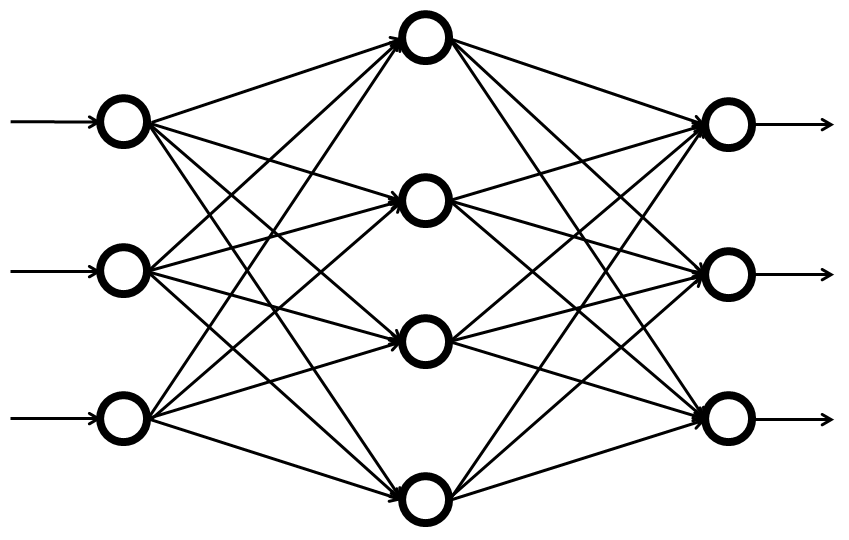
\includegraphics[width=8cm]{pic/dnn_sample.png}
\end{center}

\footnote{\url{http://nkdkccmbr.hateblo.jp/entry/2016/10/06/222245}より}
\end{frame}

\begin{frame}[fragile]{ニューラルネットワークの雰囲気}
  \begin{itemize}
    \item $\bullet$: ユニット
    \item $\bullet$の列: 層
    \item 層を重ねて予測をする.
  \end{itemize}
\end{frame}

\begin{frame}[fragile]{二層のパーセプトロンの定義}

\begin{screen}
\begin{dfn}
以下を満たすものを二層のパーセプトロンといいます.
\begin{itemize}
\item 入力: $x_1, x_2$
\item パラメータ: $w_1, w_2, \theta$
\item 出力:
\begin{equation*}
y = \left\{
\begin{array}{ll}
0 & w_1 x_1 + w_2 x_2 < \theta \\
1 & w_1 x_2 + w_2x_2 \ge \theta
\end{array}
\right.
\end{equation*}
\end{itemize}
\end{dfn}
\end{screen}
\end{frame}


\begin{frame}[fragile]{二層のパーセプトロンの性質}
\begin{itemize}
\item 実現できるもの
  \begin{itemize}
  \item AND
  \item OR
  \item NAND
  \end{itemize}
\item 実現できないもの
   XOR
\end{itemize}

\textbf{注意}: 入力は0,1のみを考える
\end{frame}

\begin{frame}[fragile]{AND}

実現例
\begin{itemize}
  \item $w_1 = w_2 = 0.5$
  \item $\theta = 0.7$
\end{itemize}

実際計算してみる
\begin{itemize}
\item $(x_1, x_2)$が(0,0),(1,0),(0,1)のときは高々0.5
\item (1,1)のときは1となります.
\item $\theta$の条件を考えると確かに`AND`.
\end{itemize}

\end{frame}

\begin{frame}[fragile]{OR}

実現例
\begin{itemize}
  \item $w_1 = w_2 = 0.5$
  \item $\theta = 0.3$
\end{itemize}
実際計算してみると

\begin{itemize}
\item $(x_1, x_2)$が(1,1),(1,0),(0,1)のときは少なくとも0.5
\item (0,0)のときは0となります.
\item $\theta$の条件を考えると確かに`OR`.
\end{itemize}
\end{frame}


\begin{frame}[fragile]{NAND}
NANDはANDを反転させたもの. \\
実現例
\begin{itemize}
  \item $w_1 = w_2 = -0.5$
  \item $\theta = - 0.7$
\end{itemize}
\end{frame}


\begin{frame}[fragile]{二層のパーセプトロンの気持ち}
\begin{itemize}
\item 二層のパーセプトロンは超平面で分離する = 線形モデル.
\item AND/NAND/OR等のモデルはかける
\item XORのような非線形なものはかけない
\end{itemize}
\end{frame}

\begin{frame}[fragile]{XOR}
XOR: $ \{0, 1\} \times  \{0, 1\} \to  \{0, 1\}$
\begin{itemize}
  \item $(0, 1), (1, 0)$の時1
  \item $(1, 1),(0, 0)$の時0
\end{itemize}

XOR二層のパーセプトロンでは表せない \\
もし表せたとすると,矛盾することを示します.
\end{frame}


\begin{frame}[fragile]{XORが表せない証明}
$(1, 0),(0, 1)$で$w_1x_1 + w_2x_2 \ge \theta$
\begin{itemize}
    \item $(1, 0)$の時$w_1 \ge \theta$
    \item $(0, 1)$の時$w_2 \ge \theta$
\end{itemize}
$(0, 0),(1, 1)$で$w_1x_1 + w_2x_2 < \theta$
\begin{itemize}
\item $(0, 0)$の時,$0 < \theta$
\item $(1, 1)$の時,$w_1 + w_2 < \theta$
\end{itemize}

この時、$w_1 \ge \theta$,$w_2 \ge \theta$より
\begin{itemize}
\item $w_1 + w_2 \ge 2\theta$となり,$0 < \theta$より
\item $w_1 + w_2 \ge 2 \theta  > \theta$となり
\end{itemize}
$(1,1)$の場合に条件と矛盾する.
\end{frame}


\begin{frame}[fragile]{三層での表現方法}
ただし、これを三層のパーセプトロンにすれば実現できます.

\begin{equation*}
\begin{array}{ll}
s_1 =  NAND(x_1, x_2) \\
s_2 =  OR(x_1, x_2) \\
XOR(x_1, x_2) = AND(s_1, s_2)
\end{array}
\end{equation*}
\end{frame}


\begin{frame}[fragile]{XORの結果の確認}
\begin{itemize}
\item (1,1)のとき
  \begin{itemize}
  \item $s_1 = NAND(1,1) = 0, s_2 = OR(1, 1) = 1$
  \item $AND(s_1, s_2) = AND(0, 1) = 0$
  \end{itemize}
\item (1,0)のとき
  \begin{itemize}
  \item $s_1 = NAND(1,0) = 1, s_2 = OR(1, 0) = 1$
  \item $AND(s_1, s_2) = AND(1, 1) = 1$
  \end{itemize}
\item (0,1)のとき
  \begin{itemize}
  \item $s_1 = NAND(0,1) = 1, s_2 = OR(0, 1) = 1$
  \item $AND(s_1, s_2) = AND(1, 1) = 1$
  \end{itemize}
\item (0,0)のとき
  \begin{itemize}
  \item $s_1 = NAND(0,0) = 1, s_2 = OR(0, 0) = 0$
  \item $AND(s_1, s_2) = AND(1, 0) = 0$
  \end{itemize}
\end{itemize}
\end{frame}


\begin{frame}[fragile]{まとめ}
\begin{itemize}
\item AND/OR/NAND等は二層のパーセプトロンで書ける
\item XORは二層のパーセプトロンでかけない.
\item XORは三層はパーセプトロンでかくことができる
\item 三層パーセプトロンは二層パーセプトロンを必ず表せる.
\end{itemize}
\end{frame}


\begin{frame}[fragile]{演習}
XORをpythonで実装し,正解を確認してください.
\end{frame}


\section{ニューラルネットワークの定義}


\begin{frame}[fragile]{すすめ方}
ニューラルネットワークを二層、三層、多層で形式的に定義する.

\end{frame}


\begin{frame}[fragile]{二層のニューラルネットワークの定義}
行列$W_1 \in M_{n_0 n_1}(\mathbb{R})$とベクトル$b_1  \in \mathbb{R}^{n_1}$と$\sigma:\mathbb{R}^{n_1}  \to \mathbb{R}^{n_1}$が存在し,

\begin{equation*}
F = \sigma \circ f_{W_1,b_1}
\end{equation*}

と書ける時,関数$F:\mathbb{R}^{n_0} \to \mathbb{R}^{n_1}$を \textbf{二層のニューラルネットワーク}という.
ただし,$f_{W_1,b_1}:\mathbb{R}^{n_{0}} \to \mathbb{R}^{n_1}$は$ x \mapsto W_ix+b_i$で定める写像である.
\end{frame}


\begin{frame}[fragile]{Softmax回帰は二層のニューラルネットワーク}
$x \in \mathbb{R}^2, w \in \mathbb{R}^{2 \times 2}$とする.$f:  \mathbb{R}^2 \to  \mathbb{R}^2$に対して,

\begin{equation*}
  f(x) = \mathrm{softmax}(w \cdot x)
\end{equation*}

\textbf{注意}: 分類の場合はさらに$\mathrm{argmax}$で値域を変えて場合もある.
\end{frame}


\begin{frame}[fragile]{三層のニューラルネットワークの定義}
行列$W_1 \in (\mathbb{R}^{n_0 \times n_1}),W_2 \in (\mathbb{R}^{n_1 \times n_2})$とベクトル$b_1  \in \mathbb{R}^{n_1} ,b_2 \in \mathbb{R}^{n_2}$と$ \sigma:\mathbb{R}^{n_2}  \to \mathbb{R}^{n_2}$が存在し,
\begin{equation*}
F = \tau \circ f_{W_2,b_2} \circ \sigma \circ f_{W_1,b_1}
\end{equation*}

と書ける時,関数$F:\mathbb{R}^{n_0} \to \mathbb{R}^{n_2}$を \textbf{三層のニューラルネットワーク}という.
ただし,$f_{W_i,b_i}:\mathbb{R}^{n_{i-1}} \to \mathbb{R}^{n_i}$は$ x \mapsto W_ix+b_i$で定める写像である.
\end{frame}


\begin{frame}[fragile]{ニューラルネットワークの絵(再掲)}
![](https://cdn-ak.f.st-hatena.com/images/fotolife/n/nkdkccmbr/20161006/20161006215155.png)
この画像は[人工知能であそぶ](http://nkdkccmbr.hateblo.jp/entry/2016/10/06/222245)で公開されていたものを使わせていただきました.

\end{frame}


\begin{frame}[fragile]{ニューラルネットワークのグラフ構造}
\begin{itemize}
\item グラフは点と線の組
\item $\mathbb{R}^n \to \mathbb{R}^{m}$の場合,n個の点とm個の点を結ぶ
\item ニューラルネットワークの絵はグラフ
  \begin{itemize}
  \item 単純グラフ(ループ、多重辺のない)
  \item 重み付き(重みが行列の掛け算に相当)
  \item 活性化関数を加えることも
  \end{itemize}
\end{itemize}

\end{frame}


\begin{frame}[fragile]{$L$層ニューラルネットワーク}
\begin{itemize}
  \item 2層3層のニューラルネットワークから層を増減させることで$L$層ニューラルネットワークを定義できる.
  \item 入力層と出力層が必要なので最低でも2層は必要.
  \item グラフとしては行列の重みしかないが、実際には2層,3層と同様に活性化関数がある.
\end{itemize}
\end{frame}


\begin{frame}[fragile]{隠れ層の活性化関数}
以下が有名
\begin{itemize}
\item sigmoid :$\sigma(x) = \frac{1}{1 + e^{-x}}$
\item: $ReLU(x) = \max\{x, 0\}$
\end{itemize}

だが、sigmoidは勾配消失問題があるため、ReLUが実質一強状態.
ReLUの亜種はいくつかある。
\end{frame}


\begin{frame}[fragile]{演習}
以下を微分せよ.ただし、$ReLU$は$x=0$では劣微分を求めてください.
\begin{itemize}
\item  sigmoid :$\sigma(x) = \frac{1}{1 + e^{-x}}$
\item ReLU: $ReLU(x) = \max\{x, 0\}$
\end{itemize}
\end{frame}


\section{深層学習の表現能力}

\begin{frame}[fragile]{機械学習モデルの表現能力とは}
\begin{itemize}
\item どれだけ難しい問題だとしても学習できるか
\item つまり,うまいパラメータをとったときにどの精度になるか
  \begin{itemize}
  \item 分類:空間を分割できる数がどれだけ多いか?
  \item 回帰:真の関数との誤差≒損失をどこまで小さくできるか?
  \end{itemize}
\end{itemize}
\end{frame}


\begin{frame}[fragile]{万能近似定理}
一言でいうと,ニューラルネットワークは全ての連続関数を近似できる.
厳密に言うと,
\begin{theorem}
定義域がコンパクトな連続関数全体の空間上,$\sigma,\tau$にシグモイド関数を取った三層のニューラルネットワーク全体のなす集合はsupノルムが定める位相に対して稠密である.
\end{theorem}
\end{frame}


\begin{frame}[fragile]{万能近似定理の用語}
\begin{itemize}
\item supノルムが定める位相: 関数の間の距離を定める方法の一つ.
  関数同士の近さを図る場合に成分ごとの絶対値$|f(x)_i-g(x)_i|$の最大値で定めたもの.
\item 稠密: 全てとは限らないが、いくらでも近いものがある.
  例) 有理数は実数の中で稠密.
\item コンパクト: 有界な閉集合のこと.例えば $[0, 1]$
\end{itemize}
\end{frame}


\begin{frame}[fragile]{深層の強み1}
Montufar, Pascanu, Cho, Bengio(2014年)
\begin{theorem}
隠れ層の活性化関数がReLUのニューラルネットワークを考える.
\begin{itemize}
  \item 隠れ層の数を$L$
  \item 隠れ層のユニットの数を$n$
  \item 入力の次元を$d$
\end{itemize}
このとき,入力空間は最大で$\displaystyle\left(\frac{n}{d}\right)^{L-1}\sum_{i=0}^{d}\binom{n}{i}$個の領域に分割可能
\end{theorem}

\begin{itemize}
\item つまり、これだけ分類できる可能性がある.
\item 層の数に指数的に伸びる
\item ユニットの数に対しては多項式的な伸びる
\end{itemize}
\end{frame}


\begin{frame}[fragile]{深層の強み2}
\begin{theorem}[Imaizumi, Fukumizu(2018年]
十分なユニット数と十分な深さをもつ深層ニューラルネットワークは、不連続な関数、特に区分的に滑らかな関数を表現できる。
\end{theorem}

区分的に滑らかな関数はRBFカーネルのサポートベクトルマシンでは表現できず,真に強い、
\end{frame}


\section{ニューラルネットワークの学習方法}


\begin{frame}[fragile]{学習の基本的な考え方}
\begin{itemize}
\item 損失が最小になるようにパラメータを調整する
\item 深層学習の学習の特徴
  \begin{itemize}
  \item パラーメータが多い
  \item データが多い(少ないと学習できないことも多い)
  \item データもパラメータも多いので、勾配降下の計算が大変
    \begin{itemize}
    \item 空間(メモリ的にも)
    \item 時間(計算時間的にも)
    \end{itemize}
  \end{itemize}
\item 方針
  \begin{itemize}
  \item 学習のアルゴリズムを工夫する(誤差逆伝播法)
  \item 学習データを工夫する(確率的勾配降下)
  \end{itemize}
\end{itemize}
\end{frame}

\section{学習のアルゴリズムを工夫する(誤差逆伝播法)}

\begin{frame}[fragile]{誤差逆伝播法}
\begin{itemize}
\item 勾配降下では損失関数のパラメータでの偏微分を行う
\item ニューラルネットワークでは偏微分すると後ろの層の偏微分が出てくる.
\item 後ろから計算させて計算量を減らすことを誤差逆伝播法という
\end{itemize}
\end{frame}


\begin{frame}[fragile]{誤差逆伝搬の計算方法}
$\ell = (y - \sigma \circ W^c \circ \sigma \circ W^{b} \circ \sigma \circ W^{a}(x))^2$の場合を考える
\begin{itemize}
  \item パラメータは$W^c, W^b, W^a$
  \item $f^c(x) = (\sigma \circ W^cx)$
  \item $f^b(x) = (\sigma \circ W^bx)$
  \item $f^a(x) = (\sigma \circ W^ax)$
  \item $u_a = W^ax, z_a = f^a(x)$
  \item $u_b = W^bz_a, z_b = f^b(z_a)$
  \item $u_c = W^cz_b, z_c = f^c(z_b)$
  \item $\ell = (y - f_c(z_b))^2 = (y - f_c(f_b(z_a))^2 = (y - f_c(f_b(f_a(x))))^2$
\end{itemize}
\end{frame}


\begin{frame}[fragile]{偏微分の計算}
\begin{align*}
\frac{\partial \ell}{\partial W^c_{11}} & =  \frac{\partial \ell}{\partial z_c}\cdot \frac{\partial f_c}{\partial W^c_{11}}= 2(y - z_c) \cdot \frac{\partial f_c}{\partial W^c_{11}} \\
  & = 2(y- z_c) \cdot \frac{\partial \sigma}{\partial u_c} \frac{\partial u_c}{\partial W^c_{11}} = 2(y-z_c)(\sigma(u_c)(1 - \sigma(u_c))(x_1)
\end{align*}
\begin{equation*}
\frac{\partial \ell}{\partial W^b_{11}} =  \frac{\partial \ell}{\partial z_c}\cdot  \frac{\partial f_c}{\partial z_b}\frac{\partial f_b}{\partial W^b_{11}}
\end{equation*}
\begin{itemize}
  \item 右辺の初項は上の偏微分計算の中で求めている.
  \item 毎回ラスト2項だけ新しく計算して求めていく.
\end{itemize}

\begin{itemize}
\item Jacobi行列の積になっていることには注意
\end{itemize}
\end{frame}


\begin{frame}[fragile]{演習}
実際に3層のNNに対して,誤差逆伝搬を使い,損失の微分を計算しよう.
\begin{itemize}
\item 活性化関数は全て$sigmoid$
\item 入力(1,1), 出力(1,0)
\item 損失は二乗誤差
\end{itemize}
\begin{equation*}
W_1 = \begin{pmatrix}
2 & 3 \\
1 & 4 
\end{pmatrix}
\end{equation*}

\begin{equation*}
W_2 = \begin{pmatrix}
3 & -1 \\
0 & 4 
\end{pmatrix}
\end{equation*}
\end{frame}

\section{学習データを工夫する(確率的勾配降下)}
\begin{frame}[fragile]{確率的勾配降下}
\begin{itemize}
\item データを小さいサイズに分割して、勾配降下させる.
\item 全てのデータは使わない.
\item 厳密には
  \begin{itemize}
  \item 確率的勾配降下はサイズが一つ
  \item バッチ型勾配降下はサイズが1以上をさす
  \end{itemize}
\item PytorchなどのクラスはバッチでもSGDになる.
  (バッチ型に対してSGDということも多い.)
\end{itemize}
\end{frame}


\begin{frame}[fragile]{普通の勾配降下法(復習)}
\begin{itemize}
\item 例えばデータが1000個あるとする
\item 普通の損失は$L(w;D)  = \sum_{i = 1}^{1000} \ell(w, x_i, y_i)$
\item これの勾配を計算する.
\item データが多すぎるとメモリや計算時間で限界が来る.
\end{itemize}
\end{frame}


\begin{frame}[fragile]{確率勾配降下法}
例えばデータが1000個あるとする。確率的勾配降下はこれをデータを10個の組にランダムに分割する. \\
$j=1$から10まで分割する場合
\begin{equation*}
  L_j(w;D)  = \sum_{i = 100j +1}^{100j + 100} \ell(w, x_i, y_i)
\end{equation*}
\begin{itemize}
\item  メリット: 一度の計算が小さくなる.
\item 注意: データが毎回変わるため、パラメータが同じでも損失の値が変わる.
\end{itemize}
\end{frame}


\begin{frame}[fragile]{確率的勾配降下の理論保証}
  TBD
\end{frame}

\begin{frame}[fragile]{確率的勾配降下法の亜種}
方式例
\begin{itemize}
  \item RMSProp
  \item Adagrad
  \item ADAM
\end{itemize}
現状
\begin{itemize}
  \item ADAMがいいSGDがいい等が度々議論(論文)になる
  \item 画一的な結論は出ていない.
\end{itemize}
\end{frame}

\section{ニューラルネットワークのチューニング}

\begin{frame}{勾配消失問題}
Sigmoidのは微分は真に1未満になる.
そのためSigmoidを活性化関数とすると微分が非常に小さい値になることもある.
\begin{itemize}
  \item  $\sigma(x)$の微分は$\sigma(x)(1 - \sigma(x))$
  \item $\sigma(x) < 1$よりどんどん小さくなる.
\end{itemize}
これを勾配消失問題という. 

$\Rightarrow$ 対策:ReLUのような関数を使う.
\end{frame}


\begin{frame}[fragile]{チューニングの方法}
Overfitting
\begin{itemize}
  \item 重み減衰
  \item Dropout
  \item ノイズ混入
  \item Early Stopping
\end{itemize}
勾配消失問題
\begin{itemize}
  \item BatchNormalization
\end{itemize}
\end{frame}


\begin{frame}[fragile]{重み減衰}
以下のようにパラメータを更新すること
\begin{equation*}
  w_{t+1} =  w_{t} - \eta \frac{\partial \ell}{\partial w}(w_t) - \eta \lambda w_t
\end{equation*}
$L^2$正則化に相当する.
つまり,ロスを$\ell$ではなく$\ell + \lambda ||w||^2$にしたもの.

\begin{minted}[frame=lines, fontsize=\footnotesize, breaklines=true, bgcolor=black]{python}
optimizer = torch.optim.SGD(model.parameters(), lr=0.1, momentum=0.9, weight_decay=0.01)
optimizer.zero_grad()
loss_fn(model(input), target).backward()
optimizer.step()
\end{minted}
\end{frame}


\begin{frame}[fragile]{Dropout}
- ランダムに入力を0に変更する.

\begin{minted}[frame=lines, fontsize=\footnotesize, breaklines=true, bgcolor=black]{python}
m = nn.Dropout(p=0.2)
input = torch.randn(20, 16)
output = m(input)
print(output)
\end{minted}

\end{frame}


\begin{frame}[fragile]{Batch Normalization}
- バッチ内で入力を平均0,分散1のminibatchに変換する.
\begin{minted}[frame=lines, fontsize=\footnotesize, breaklines=true, bgcolor=black]{python}
# With Learnable Parameters
m = nn.BatchNorm1d(100)
# Without Learnable Parameters
m = nn.BatchNorm1d(100, affine=False)
input = torch.randn(20, 100)
output = m(input)
\end{minted}
- 推論時は学習時の変換に合わせる.

\end{frame}
\begin{frame}[fragile]{Early Stopping}
- 誤差が十分に小さい場合に学習をやめる.
\begin{minted}[frame=lines, fontsize=\footnotesize, breaklines=true, bgcolor=black]{python}
from torchsample.callbacks import EarlyStopping

callbacks = [EarlyStopping(monitor='val_loss', patience=5)]
model.set_callbacks(callbacks)
\end{minted}
\end{frame}
\begin{frame}[fragile]{ノイズ混入}
\begin{itemize}
\item 敢えて誤ったデータを入れると適切に正則化する場合がある.
\item 正直いって悲しいが割とある...
\end{itemize}
\end{frame}


\begin{frame}[fragile]{演習}
- PytorchでDNNを使いMNISTの分類を行ってください.

\end{frame}
\begin{frame}[fragile]{今後作りたいなと思っているもの}
\begin{itemize}
\item CNN(AlexNet): CNNの基本
\item ReSNet: CNNの重要なもの
\item M2Det: 物体検出で大事そうなので.
\item GAN: 生成モデル一個ぐらいは
\item DeepFM: レコメンドの一つ
\item Collaborative Metric Learning: レコメンドの一つ
\item Are We Really Making Much Progress? A Worrying Analysis of Recent Neural Recommendation Approaches (RecSys 2019): RecSys 2019のトップ論文
\end{itemize}
\end{frame}

\section{ChainerのPythonコードを追う}

\begin{frame}[fragile]{DeepLearningの処理をおう}
対象
\begin{itemize}
\item  Linear: (行列をかける)
\item SGD: (勾配降下)
\end{itemize}

Chainerにした理由
\begin{itemize}
\item 雰囲気でも追える
\item 他はPython部分に処理が少ない.
\end{itemize}
\end{frame}


\begin{frame}[fragile]{Linear}
\url{https://github.com/chainer/chainer/blob/eb8dee82942ef3c1b9ef6f89d7fe93ed8e6bb819/chainer/functions/connection/linear.py#L13}

\begin{minted}[frame=lines, fontsize=\footnotesize, breaklines=true, bgcolor=black]{python}
class LinearFunction(function_node.FunctionNode):
    #intel cpuでの高速化
    _config_use_ideep = None
    _supports_static_optimizations = True
\end{minted}
以降は関係ない部分は省略する.
\end{frame}


\begin{frame}[fragile]{forward}
\begin{minted}[frame=lines, fontsize=\footnotesize, breaklines=true, bgcolor=black]{python}
def forward(self, inputs):
    if len(inputs) == 3:
        x, W, b = inputs
    else:
        (x, W), b = inputs, None
    xp = backend.get_array_module(x)
    y = xp.empty((x.shape[0], W.shape[0]), dtype=x.dtype)
    # 行列をかける
    self.static_linear_no_bias(xp, x.dtype == W.dtype, inputs=[x, W], outputs=[y])
    if len(inputs) == 3:
        self.static_add_bias(inputs=[b], outputs=[y])
    
    self.retain_inputs((0, 1))  # b is not retained
    return y,
\end{minted}
\end{frame}
        

\begin{frame}[fragile]{static\_linear\_no\_bias}
\begin{minted}[frame=lines, fontsize=\footnotesize, breaklines=true, bgcolor=black]{python}
@static_code
def static_linear_no_bias(self, xp, optimized, inputs, outputs):
    x, W = inputs
    y = outputs[0]

    if optimized:
        # Note: We can only call this function when both x and W
        # have the same dtype. Otherwise, the output type (for y)
        # may not be as expected (i.e., not the same dtype as x).
        xp.dot(x, W.T, out=y)
    else:
        y[:] = x.dot(W.T).astype(x.dtype, copy=False)
\end{minted}
\end{frame}


\begin{frame}[fragile]{結局やっていること}
\begin{itemize}
\item ただ$x, W$の行列をかけている
\item $x$がバッチになっても対応している.
\item バイアスあり、なしともに対応している.
\item 高速化の工夫をしている.
\end{itemize}


\end{frame}
\begin{frame}[fragile]{backward}
\begin{minted}[frame=lines, fontsize=\footnotesize, breaklines=true, bgcolor=black]{python}
def backward(self, indexes, grad_outputs):
    x, W = self.get_retained_inputs()
    gy, = grad_outputs
    ret = []
    
    if 0 in indexes:
        gx, = LinearGradData().apply((W, gy))
        ret.append(chainer.functions.cast(gx, x.dtype))
    if 1 in indexes:
        gW, = LinearGradWeight(W.dtype).apply((x, gy))
        ret.append(chainer.functions.cast(gW, W.dtype))
    if 2 in indexes:
        gb = chainer.functions.sum(gy, axis=0)
        ret.append(gb)

    return ret
\end{minted}

\end{frame}


\begin{frame}[fragile]{get\_retaind\_inputs()}
\begin{minted}[frame=lines, fontsize=\footnotesize, breaklines=true, bgcolor=black]{python}
    def get_retained_inputs(self):
        retained_inputs = []
        for index in self._input_indexes_to_retain:
            input = self.inputs[index]
            if input.data is None:
                retained_inputs.append(None)
            else:
               retained_inputs.append(input.get_variable())
        return tuple(retained_inputs)
\end{minted}
\end{frame}


\begin{frame}[fragile]{SGD}
\begin{minted}[frame=lines, fontsize=\footnotesize, breaklines=true, bgcolor=black]{python}
class SGD(optimizer.GradientMethod):
    """Vanilla Stochastic Gradient Descent.
    Args:
        lr (float): Learning rate.
    """

    def __init__(self, lr=_default_hyperparam.lr):
        super(SGD, self).__init__()
        self.hyperparam.lr = lr

    lr = optimizer.HyperparameterProxy('lr')

    def create_update_rule(self):
        return SGDRule(self.hyperparam)
\end{minted}
\end{frame}


\begin{frame}[fragile]{SGDRule 初期化}
\begin{minted}[frame=lines, fontsize=\footnotesize, breaklines=true, bgcolor=black]{python}
class SGDRule(optimizer.UpdateRule):

    """Update rule of vanilla stochastic gradient descent.
    """
    is_elementwise = True

    _kernel = None

    def __init__(self, parent_hyperparam=None, lr=None):
        super(SGDRule, self).__init__(
            parent_hyperparam or _default_hyperparam)
        if lr is not None:
            self.hyperparam.lr = lr
\end{minted}
\end{frame}


\begin{frame}[fragile]{SGDRule 更新}
パラメータの更新を行う.

\begin{minted}[frame=lines, fontsize=\footnotesize, breaklines=true, bgcolor=black]{python}
    def update_core_cpu(self, param):
        grad = param.grad
        if grad is None:
            return
        if isinstance(param.data, intel64.mdarray):
            param.data.inplace_axpby(1.0, -self.hyperparam.lr, grad)
        else:
            # パラメーターを更新した
            param.data -= self.hyperparam.lr * grad
\end{minted}
\end{frame}

%\section{Pytorch 入門}

\begin{frame}[fragile]{ここで学ぶこと}
 DeepLearningの基本的な実装方法
 \begin{itemize}
  \item Pytorchの基本的な型
  \item DLのプログラムの基本的な処理方法
  \item 各コンポーネントで使われるクラス.
 \end{itemize}

\end{frame}
\begin{frame}[fragile]{機械学習で必要な操作}
\begin{itemize}
\item データの前処理
\item 学習
\item 推論
\item 評価
\end{itemize}

\end{frame}
\begin{frame}[fragile]{深層学習エンジニアがやること}
https://<!-- slide -->
www.slideshare.net/pfi/20171212-gtc-pfnchainer

![](https://image.slidesharecdn.com/20171212gtcpfnchainer-171215022416/95/20171212-gtc-pfnchainer-6-638.jpg?cb=1513305240)

\end{frame}
\begin{frame}[fragile]{フレームワークで考えること}
どのようにネットワークを記述するか?
\begin{itemize}
  \item 複雑なモデルを簡単に記述するには
  \item 実装ミスを減らすには
  \item デバッグするには
  \item モデル以外も簡単に書くには
\end{itemize}

どのように最適化するか
\begin{itemize}
  \item 自動微分等の最適化プロうグラムを実行
  \item いかに高速・省メモリで実行するるか
\end{itemize}
\end{frame}

\begin{frame}[fragile]{個人的な見解}
\begin{itemize}
\item ネットワークの定義方法はどこも近づいている.
\item 最近はそれ以外で勝敗が決まっている気がする
  \begin{itemize}
  \item  前処理の書きやすさ
  \item 結果の可視化が楽か
  \item ユーザの多さ
    \begin{itemize}
    \item  バグの少なさ
    \item 最先端ライブラリの再現実装数
    \end{itemize}
  \end{itemize}
\end{itemize}

とはいえ,好きなものを使えば良い
\end{frame}


\begin{frame}[fragile]{個人的な好み}
\begin{itemize}
\item  Chainer
  \begin{itemize}
  \item  ソースコードが最も美しい.
  \item 困ったらソースを読む.
  \end{itemize}
\item Pytorch
  \begin{itemize}
  \item  ChainerからForkしたので思想が近い
  \item  Nvidia,Facebookも使っており人口が多い
  \end{itemize}
\item Tensorflow
   \begin{itemize}
    \item Python2系色が強い
    \item ソースコード読むのが地獄だった...
   \end{itemize}
\end{itemize}
\end{frame}


\begin{frame}[fragile]{Chainerの現状}
\begin{itemize}
\item 開発を止めるとのこと。
\item お疲れさまです。
\end{itemize}
\end{frame}


\begin{frame}[fragile]{実際のコーディングに関して}
\begin{itemize}
\item フレームワークでできる範囲の場合、モデルの作成は慣れればすぐ
\item 変化は早いので都度ドキュメント確認
\item 勉強する時もドキュメントとソースを読んだ方がよい.
\item 実際使う場合はデータの前処理が重い
\item メモリや再現性が大変なことも...
\end{itemize}
\end{frame}


\begin{frame}[fragile]{プログラミングなれていない人は}
\begin{itemize}
\item 恐れずにPytorchのTutorialをやりましょう.
\item わからない場合は一緒に調べましょう.
\end{itemize}
\end{frame}


\begin{frame}[fragile]{機械学習フレームワークを使ってやること}
我々が実装するもの
\begin{itemize}
  \item データの前処理
  \item 仮説(機械学習モデル)
  \item 損失関数
\end{itemize}
実装せずに行うこと
\begin{itemize}
  \item 学習して、最適な$w$を求めること.
  \item 裏では微分計算が行われる( \textbf{自動微分})
\end{itemize}
\end{frame}


\begin{frame}[fragile]{Pytorchの環境構築方法}
デフォルトで入っているもの
\begin{itemize}
  \item Kaggle Kernel
  \item Google Collaboratory
\end{itemize}
Jupyter Notebookの場合はインストールが必要
  公式ページで確認.
  \url{https://pytorch.org/}
\end{frame}


\begin{frame}[fragile]{Pytorchでよく使うもの}
\begin{itemize}
\item Tensor: Pytorch用の多次元配列 \\
  入力: $x$, パラメータ: $w$,
\item Dataset/Dataloader \\
  データの前処理、読み込み
\item nn.Module \\
  ニューラルネットワーク
\item optim \\
  最適化アルゴリズム
\end{itemize}
一つずつ見ていく.
\end{frame}


\begin{frame}[fragile]{Tensor}
\begin{itemize}
  \item numpy.ndarrayのような多次元配列
  \item numpyと違って勾配の情報もある.
  \item Pytorchの入力はTensorにする必要がある.
\end{itemize}

Tensorの機械学習的な意味
\begin{itemize}
  \item 機械学習では3次元以上の多次元配列をさす事が多い.
  \item 数学的にはベクトル空間や加群の積として定義される
\end{itemize}

\end{frame}
\begin{frame}[fragile]{Tensorになれる}

\begin{minted}[frame=lines, fontsize=\footnotesize, breaklines=true, bgcolor=black]{python}
# uninitializedなので、0とは限らない
x = torch.empty(5, 3)
print(x)
# 乱数の生成
x = torch.rand(5, 3)
print(x)
# zero
x = torch.zeros(5, 3, dtype=torch.long)
print(x)
\end{minted}
\end{frame}


\begin{frame}[fragile]{Tensorになれる}
\begin{minted}[frame=lines, fontsize=\footnotesize, breaklines=true, bgcolor=black]{python}
x = torch.tensor([5.5, 3])
print(x)
x = x.new_ones(5, 3, dtype=torch.double)      # new_* methods take in sizes
print(x)
​
x = torch.randn_like(x, dtype=torch.float)    # override dtype!
print(x)
\end{minted}

\end{frame}
\begin{frame}[fragile]{Tensorになれる}
\begin{minted}[frame=lines, fontsize=\footnotesize, breaklines=true, bgcolor=black]{python}
y = torch.rand(5, 3)
print(x + y)
​
result = torch.empty(5, 3)
torch.add(x, y, out=result)
print(result)
\end{minted}
\end{frame}


\begin{frame}[fragile]{使うパッケージのimport}
\begin{minted}[frame=lines, fontsize=\footnotesize, breaklines=true, bgcolor=black]{python}
from torchvision import datasets, transforms
import torch.nn as nn
import torch.nn.functional as F
import torch.optim as optim
\end{minted}
\end{frame}


\begin{frame}[fragile]{Dataset/Dataloader}
\begin{itemize}
\item 複雑なので、後で説明する.
\item kagglekernelはデータをDLできないので、エラーになる場合も
\end{itemize}
以下で使える
\begin{minted}[frame=lines, fontsize=\footnotesize, breaklines=true, bgcolor=black]{python}
    train_loader = torch.utils.data.DataLoader(
        datasets.MNIST('../data', train=True, download=True,
                       transform=transforms.Compose([
                           transforms.ToTensor(),
                           transforms.Normalize((0.1307,), (0.3081,))
                       ])),
        batch_size=args.batch_size, shuffle=True)
\end{minted}
\end{frame}


\begin{frame}[fragile]{ニューラルネットワークの作成}
\begin{itemize}
\item linearは行列をかける関数
\item forwardはNNの計算を実際に行う
\end{itemize}

\begin{minted}[frame=lines, fontsize=\footnotesize, breaklines=true, bgcolor=black]{python}
class Net(nn.Module):
    def __init__(self, input_size, output_size):
        super(Net, self).__init__()
        self.input_size = input_size
        self.output_size = output_size
        self.linear = nn.Linear(input_size, output_size)

    def forward(self, x):
        x = x.view(-1, self.input_size) # reshape
        return self.linear(x)
\end{minted}
\end{frame}

\begin{frame}[fragile]{パラメーター更新の設定}

```python
model = Net(input_size, output_size)
criterion = nn.CrossEntropyLoss() # 損失の定義
optimizer = torch.optim.SGD(model.parameters(), lr=learning_rate) # (確率的)勾配降下法
```


\end{frame}
\begin{frame}[fragile]{}実際の学習
```python
model.train() # 学習用のモード
for epoch, (data, target) in enumerate(train_loader): # 入力と正解
     optimizer.zero_grad() #Weightの初期化
     output = model(data) # 仮説で値代入
     loss = criterion(output, target) # 損失
     loss.backward() # 微分の計算
     optimizer.step() # パラメータの更新
     if epoch % 600 == 0:
         print('Train Epoch: {} [{}/{} ({:.0f}%)]\tLoss: {:.6f}'.format(
             epoch, epoch * len(data), len(train_loader.dataset),
             100. * epoch / len(train_loader), loss.item()))
```

\end{frame}
\begin{frame}[fragile]{}結果の評価
```python
model.eval()
test_loss = 0
correct = 0
with torch.no_grad():
    for data, target in test_loader:
        output = model(data)
        test_loss += F.nll_loss(output, target, reduction='sum').item() # sum up batch loss
        pred = output.argmax(dim=1, keepdim=True) # get the index of the max log-probability
        correct += pred.eq(target.view_as(pred)).sum().item()

test_loss /= len(test_loader.dataset)

print('\nTest set: Average loss: {:.4f}, Accuracy: {}/{} ({:.0f}%)\n'.format(
    test_loss, correct, len(test_loader.dataset),
    100. * correct / len(test_loader.dataset)))
```

\end{frame}
\begin{frame}[fragile]{}余談
今回はデータをすべて一度しか使っておらず、学習は収束していない。 そのため、何回か学習を繰り返すことで評価データの精度も向上する。

\end{frame}
\begin{frame}[fragile]{}演習
IRISのデータに対してpytorchでSoftmax回帰を実装せよ.


\end{frame}
\begin{frame}[fragile]{}結果の可視化

Tensorboard一択

\end{frame}
\begin{frame}[fragile]{}Tensorboard
```python
from torch.utils.tensorboard import SummaryWriter

# default `log_dir` is "runs" - we'll be more specific here
writer = SummaryWriter('runs/fashion_mnist_experiment_1')
dataiter = iter(trainloader)
images, labels = dataiter.next()

# create grid of images
img_grid = torchvision.utils.make_grid(images)

# show images
matplotlib_imshow(img_grid, one_channel=True)

# write to tensorboard
writer.add_image('four_fashion_mnist_images', img_grid)
```

\end{frame}
\begin{frame}[fragile]{}Tensoboardで欲しいもの
- 計算グラフ
- サンプルデータの可視化
- 訓練誤差,評価誤差
- Weightの遷移 #個人的にはあまり使ったことがない

\end{frame}
\begin{frame}[fragile]{}Tensorboardの使い方
```bash
tensorboard --logdir=runs
```
from the command line and then navigating to https://localhost:6006 should show the following.

\end{frame}
\begin{frame}[fragile]{Kaggle Kernelだと}
https://www.kaggle.com/aagundez/using-tensorboard-in-kaggle-kernels

```
%load_ext tensorboard.notebook
%tensorboard --logdir logs
```


\section{dataの前処理}

\end{frame}
\begin{frame}[fragile]{}Dataを持つクラス
- データ自体を内部に持つクラスが2つあります
  - Dataset
  - Dataloader

- Datasetは入力にするデータそのもの.
  生データを入力にし、内部的に整形して、データを保持する
- Dataloaderは実際に学習、推論する時に使われるバッチ単位のデータ

\end{frame}
\begin{frame}[fragile]{}前処理のプロセス
Pytorchの前処理としては

1. Datasetクラスでデータを整形、保持
2. そこから適切にサンプリングしてDataLoaderを作成

- データの整形、サンプリングは複雑な処理になる場合もあるため、分離されている.
  - データの整形は`transform`メソッドで行われ、
  - サンプリングは`Sampler`クラスで実行されます。

\end{frame}
\begin{frame}[fragile]{}Datasetクラス
- データを受け取るクラスです。

- 現在主に2つの種類のデータセットがあります。
  - iterable-style
  - map-style
- 参考: https://pytorch.org/docs/stable/data.html

\end{frame}
\begin{frame}[fragile]{}iterable-styleは
iterable-styleは以下が実装されていればよいようです。

```python
def __iter__(self)
```

ただ、このiteratorではsamplingなども一つに入ることになってしまうので、あまり推奨されていないのかなと思いました。

\end{frame}
\begin{frame}[fragile]{}map-style
- map-styleはlistやdictなどでkeyを元に受け取りるデータクラス.
- 以下が実装されいればよいです。
  - `__getitem__(self, index)`
    教師あり学習の場合は正解も含め返すことが多そうです。
  - `__len__(self)`
     サイズ(整数値)
- [ソースコード](https://github.com/pytorch/pytorch/blob/master/torch/utils/data/dataset.py#L8)を見ると
`__len__` に対して何か制約してるわけではなさそう.
- `Sampler`で使われるので、実質必須.

\end{frame}
\begin{frame}[fragile]{}transform
- プロトコルとしては定義されておらず。
- [Pytorchのチュートリアル](https://pytorch.org/tutorials/beginner/data_loading_tutorial.html)を見ても、使われています。

\end{frame}
\begin{frame}[fragile]{}コード例

```python

    def __init__(self, csv_file, root_dir, transform=None):
        self.landmarks_frame = pd.read_csv(csv_file)
        self.root_dir = root_dir
        self.transform = transform

    def __len__(self):
        return len(self.landmarks_frame)

    def __getitem__(self, idx):
        if torch.is_tensor(idx):
            idx = idx.tolist()

        img_name = os.path.join(self.root_dir,
                                self.landmarks_frame.iloc[idx, 0])
        image = io.imread(img_name)
        landmarks = self.landmarks_frame.iloc[idx, 1:]
        landmarks = np.array([landmarks])
        landmarks = landmarks.astype('float').reshape(-1, 2)
        sample = {'image': image, 'landmarks': landmarks}

        if self.transform:
            sample = self.transform(sample)

        return sample
```

\end{frame}
\begin{frame}[fragile]{}Transform/Sampler
- Transoform
  - データの加工をするものです。
  - 特に制限はなく必要な処理を実装すればよい
- Sampler
  - Dataに対してサンプリングする処理をするもの
  - 特に制限はなく必要な処理を実装すればよい


\end{frame}
\begin{frame}[fragile]{Dataloader}
```python
for indices in batch_sampler:
    yield collate_fn([dataset[i] for i in indices])
```
という結果を返す.

\end{frame}
\begin{frame}[fragile]{collate_fn}
\begin{itemize}
\item dataを処理するもの
\item 例えば物体検出のように入力と出力のsizeが異なる場合はで適切に処理する必要があります。
\end{itemize}

\end{frame}


\begin{frame}[fragile]{Tensorboard}
\begin{itemize}
\item 前提: 本来はtensorflow用のもの
\item pytorchでも使えるが,結果を出力するには`tensorflow`が必要(のようだ).
\item インストールは`pip install tensorflow tensorboard`でできる.
\item tensorflowはpython3.7系では動かない?
\item poetry, pipenvでは(たいていの場合に)入らない
\item gpuを使いたい場合は`tensorflow-gpu`になる.
\item インストールが複雑のため、有志がお試しください.
\end{itemize}
\end{frame}


\begin{frame}[fragile]{演習}
Alexnetを微分して,
各パラメータの更新式を記述しなさい.
\end{frame}


\begin{frame}[fragile]{演習}
\begin{itemize}
\item PytorchでMNISTを4層のDNNで学習してみてください
\item PytorchでIRISを4層のDNNで学習してみてください
\item Pytorchで以下の条件でMNISTをDNNで学習してみください
  \begin{itemize}
  \item Weight Decay 0.01
  \item BatchNormalizationあり
  \item Dropoutあり
  \item これらの差分をTensorboardで可視化する.
  \end{itemize}
\end{itemize}
\end{frame}



%\section{Graphの紹介}
%\begin{frame}{Graphの定義}
%\begin{itemize}
%\item NodeとEdgeの組 $G=(V, E)$ のこと.
%\item VはNodeの集合
%\item EはNodeとNodeの間のEdgeの集合
%\item Edgeに向きがある場合: \textbf{有向グラフ}
%\item Edgeに向きがない場合: \textbf{無向グラフ}
%\end{itemize}
%\centering
%%\fbox{
%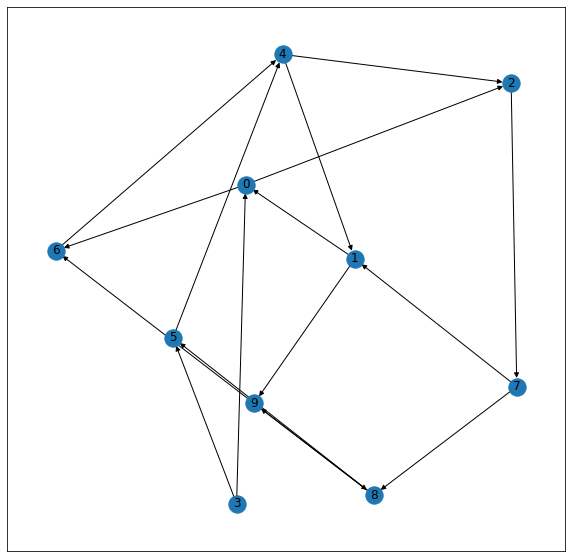
\includegraphics[width=80pt]{pic/graph.png}
%%\par\indicatewidth{right}
%\end{frame}